\documentclass[a4page,notitlepage]{report}
\usepackage{nameref}
\usepackage{gensymb}
\usepackage{color,amsmath,graphicx,subcaption,geometry,mathtools,xfrac}
\usepackage{cite}
\usepackage{mhchem}
\usepackage{tikz}
\usepackage{pgfplots}
\pgfplotsset{compat=1.12}
\usepackage{stackengine,ifthen}
\usetikzlibrary{arrows,positioning,calc,arrows.meta,patterns,fit}
\newtoggle{article}
\newtoggle{eddpathway}

\tikzset{>=Latex}
\newcommand\influx{0.5}

\newenvironment{customlegend}[1][]{
  \begingroup
  \csname pgfplots@init@cleared@structures\endcsname
  \pgfplotsset{#1}
}{
  \csname pgfplots@createlegend\endcsname
  \endgroup
}

\def\addlegendimage{\csname pgfplots@addlegendimage\endcsname}
\setlength\abovecaptionskip{6pt}
\providecommand{\abs}[1]{\lvert#1\rvert}
\providecommand{\norm}[1]{\lVert#1\rVert}

\tikzset{>=latex}
%\tikzset{metaboliteStyle/.style={rectangle,draw}}
\tikzset{metaboliteStyle/.style={}}
\definecolor{cyan}{RGB}{100,181,205}
\definecolor{blue}{RGB}{76,114,176}
\definecolor{green}{RGB}{85,168,104}
\definecolor{magenta}{RGB}{129,114,178}
\definecolor{yellow}{RGB}{204,185,116}
\definecolor{red}{RGB}{196,78,82}
\definecolor{graybg}{gray}{0.95}

\colorlet{assimcol}{green}
\colorlet{sumcolor}{yellow}

\colorlet{inputcol}{green}
\colorlet{branchout}{red}
\colorlet{branchoutfl}{red!80}
\colorlet{autocatacyc}{blue}
\colorlet{autocatacycfl}{blue!80}
\colorlet{autocataby}{cyan}

\pdfpageattr{/Group <</S /Transparency /I true /CS /DeviceRGB>>} 

\def\blendfrac{0.5}
\def\deltaang{-155}
\def\fromang{180}
\def\inputang{-40}
\def\protrude{7}
\def\arcwidth{0.3cm}
\def\highlightrad{0.2cm}
\def\autocatalrad{1.5cm}
\def\autocatalscale{1.5}

  \newcommand{\colorgradarc}[6]{%width,startang,stopang,rad,startcol,stopcol
    \pgfmathsetmacro\arcrange{#3-#2}
    \pgfmathsetmacro\progsign{\arcrange>0 ? 1 : -1}
    \pgfmathsetmacro\arcend{#3-1}
    \foreach \i in {#2,...,\arcend} {
     \pgfmathsetmacro\fracprog{\i/\arcrange-#2/\arcrange}
     \pgfmathsetmacro\col{\fracprog*100}
     \draw[color={#6!\col!#5},line width=#1] (\i-\progsign:#4)
         arc[start angle=\i-\progsign, end angle=\i+1.1*\progsign,radius=#4];
    }
  }

  \newcommand{\shadedarc}[7][\arcwidth]{%width,startang,stopang,startrad,stoprad,startcol,stopcol
    \pgfmathsetmacro\arcrange{#3-#2}
    \pgfmathsetmacro\radrange{#5-#4}
    \pgfmathsetmacro\progsign{\arcrange>0 ? 1 : -1}
    \foreach \i in {#2,...,\numexpr#3-1\relax} {
      \pgfmathsetmacro\fracprog{\i/\arcrange-#2/\arcrange}
      \pgfmathsetmacro\col{\fracprog*100}
      \draw[color={#6!\col!#7},line width=#1] (\i-\progsign:#4+\radrange*\fracprog)
  arc[start angle=\i-\progsign, end angle=\i+1.1*\progsign,radius=#4+\fracprog*\radrange];
    }
  }

  \newcommand{\coloredarc}[6][\arcwidth]{%width,startang,stopang,startrad,stoprad,startcol,stopcol
    \pgfmathsetmacro\arcrange{#3-#2}
    \pgfmathsetmacro\radrange{#5-#4}
    \pgfmathsetmacro\progsign{\arcrange>0 ? 1 : -1}
    \foreach \i in {#2,...,\numexpr#3-1\relax} {
      \pgfmathsetmacro\fracprog{\i/\arcrange-#2/\arcrange}
      \draw[color={#6},line width=#1] (\i:#4+\radrange*\fracprog)
        arc[start angle=\i, end angle=\i+1.1*\progsign,radius=#4+\fracprog*\radrange];
    }
  }

  \newcommand{\preassim}[5]{%width, startang, stopang, rad, col
    %\pgfmathsetmacro\thirdarc{#3/3-#2/3}
    \pgfmathsetmacro\halfarc{#3/2-#2/2}
    %\draw[color={#5},line width=#1] (#2:#4)
    %    arc[start angle=#2, end angle=#2+\thirdarc,radius=#4];
    \draw[color={autocatacyc},line width=#1] (#3:#4)
        %arc[start angle=#3, end angle=#3-\thirdarc,radius=#4];
        arc[start angle=#3, end angle=#3-\halfarc,radius=#4];
    %\pgfmathsetmacro\startshade{#2+\thirdarc}
    %\pgfmathsetmacro\endshade{#3-\thirdarc}
    \pgfmathsetmacro\startshade{#2}
    \pgfmathsetmacro\endshade{#3-\halfarc}
    \colorgradarc{#1}{\startshade}{\endshade}{#4}{#5}{autocatacyc}
  }

  \newcommand{\postassim}[6]{%width,startang,stopang,rad,col,ratio
    \pgfmathsetmacro\halfarc{#3/2-#2/2}
    \pgfmathsetmacro\endshade{#3-\halfarc}
    \colorgradarc{#1*#6}{#2}{\endshade}{#4+#1*#6/2-#1/2}{autocatacyc}{#5}
    \draw[color={#5},line width=#1] (\endshade:#4)
        arc[start angle=\endshade, end angle=#3,radius=#4];

    \pgfmathsetmacro\arcrange{-\halfarc}
    \pgfmathsetmacro\outstart{\endshade+180}
    \pgfmathsetmacro\progsign{\arcrange>0 ? 1 : -1}
    \pgfmathsetmacro\arcend{\outstart+\arcrange-\progsign}
    \begin{scope}[shift={(\endshade:2*#4+#1*#6/2)}]
      \colorgradarc{#1*#6-#1}{\outstart}{\arcend}{#4}{#5}{white}
    \end{scope}
  }

  \newcommand{\assim}[5]{%width,startang,deltaang,rad,ratio
    \pgfmathsetmacro\assimstart{#2+180}
    \begin{scope}[shift={(#2:2*#4+#1*#5/2)}]
      \colorgradarc{#1*#5-#1}{\assimstart}{\assimstart+#3}{#4}{autocatacyc}{assimcol}
    \end{scope}
  }

  \newcommand{\arrowhead}[4]{%width,startang,rad,col
  \fill[#4] (#2+1:#3-#1/2) arc (#2+1:#2:#3-#1/2)
       -- (#2-\protrude:#3) -- (#2:#3+#1/2) arc (#2:#2+1:#3+#1/2) -- cycle;
     }
  \newcommand{\revarrowhead}[4]{%width,startang,rad,col
  \fill[#4] (#2-1:#3-#1/2) arc (#2-1:#2:#3-#1/2)
       -- (#2+\protrude:#3) -- (#2:#3+#1/2) arc (#2:#2-1:#3+#1/2) -- cycle;
     }


\input{plos_constants.tex}

\toggletrue{article}
\toggletrue{thesis}
\togglefalse{eddpathway}

\tikzset{
  invisible/.style={opacity=0},
  visible on/.style={}
}
\title{Passive effects in molecular biology systems}
\author{Uri Barenholz}

\date{}
%\newcommand{\beginsupplement}{%
%        \setcounter{table}{0}
%        \renewcommand{\thetable}{S\arabic{table}}%
%        \setcounter{figure}{0}
%        \renewcommand{\thefigure}{S\arabic{figure}}%
%    }
\usepackage{pgfplotstable}
\begin{document}
    \newlength\gridsize;
    \pgfmathsetlength{\gridsize}{8cm};
    \newlength\plotwidth;
    \pgfmathsetlength{\plotwidth}{4.6cm};
    \newlength\plotheight;
    \pgfmathsetlength{\plotheight}{4.5cm};



\abstract{
    Molecular biology systems are complex.
    They must function in the face of multiple challenges: varying temperatures, fluctuating food supply, competition with other species and more.
    To survive and prosper, such systems have complex designs, accompanied by extensive regulation mechanisms, fine tuning their operation to ensure proper function.
    My research focuses on the system wide effects, implications, and passive outcomes of both the system design and the regulatory mechanisms.
    Specifically, I use simple models to extract testable, system wide implications emerging from the requirements of the models, then use multi-omics data to test the models predictions on living systems.

    This work spans two different domains of molecular biology: gene expression and metabolic network topology.
    In metabolism I focus on the dynamics of autocatalytic cycles, constructs that are more common than one might naively expect even in central carbon metabolism.
    Analyzing the constraints resulting from the need to maintain a functioning autocatalytic cycle points at inherent inefficiencies in both the kinetic parameters of enzymes, and in an almost obligatory requirement for over expression of key enzymes involved in shuttling metabolites out of the autocatalytic cycle.
    In gene expression patterns I show that the interplay between growth rate and active regulation patterns implies an increased concentration with growth rate as a default side-effect for non-regulated genes.
    These analyses help unveil the underlying principles and logic behind observed phenomena in these two domains, as well as predict the behavior of synthetically engineered biological systems, assisting in their design towards proper function.
}
\newpage
\section*{Acknowledgments}
\paragraph{To Prof. Ron Milo}
For opening the door to the fascinating world of biology to me.
For your constant pursue of perfection and simplicity.
For teaching me how science should be done and guiding me in learning the fundamentals of scientific work.
For your patience, support, and uncompromising commitment to excellence.
For promoting science that focuses on addressing burning issues humanity faces.
\paragraph{To the Milo lab members at present and in the past}
An extraordinary cadre of talented and committed people who have always provided good advice, and were willing to support me in my research at all times, helping me take it into higher levels.
Who create a great atmosphere to be part of, and who, by their complementing skills and expertise, highlight the power of cooperation and mutual exchange of ideas in doing science.
\paragraph{To the Weizmann Institute of Science and the Feinberg Graduate School}
That support innovative research by creating an amazing environment focused on facilitating productive scientific research and interaction.
Maintaining a welcoming, green and vast campus, where one can wander in search of ideas and meditate.
For avoiding unnecessary bureaucracies and providing unusual flexibility, demonstrating the institute's spirit of commitment to scientific excellence.
\paragraph{And especially to Hilla, my wife}
For her endless support and encouragement, especially during harder periods of uncertainty, doubt, and frustration.
For being by my side throughout this journey.

\newpage
\tableofcontents
\newpage
\chapter{Autocatalytic cycles stability constrains kinetic parameters of enzymes}
\section{Introduction}
    Autocatalysis is generally defined as a setup in which one of the products of a chemical reaction is also a reactant in the same, or coupled reaction (see, for example, \cite{Steinfeld1999-iw}).
    Naively, one can then consider them as parts of the catalyst and not part of the reaction.
    A metabolic cycle is a set of reactions and corresponding metabolites that can be ordered in such a way that one of the products of each reaction is a substrate of the following reaction, with a product of the last reaction serving as a substrate for the first reaction.
    Metabolic cycles allow metabolites external to the cycle to serve as additional reactants or products of the reactions of the cycle.
    A metabolic cycle is autocatalytic if traversing the reactions that form the cycle increases the amount of the metabolites forming it.
    Surprisingly, autocatalytic cycles can be an essential building block of optimal metabolic networks \cite{Riehl2010-yh}.

    Autocatalytic cycles present specific metabolic control challenges as their inherent feed-back nature makes them susceptible to instabilities such as divergence or drainage of their intermediate metabolites \cite{Fell1999,Reznik2010-te}.
    Understanding the unique constraints that operating metabolic autocatalytic cycles impose is therefore essential for realizing limitations of existing metabolic networks, as well as for the introduction of modifications to them in synthetic biology metabolic engineering applications.

    The importance of autocatalytic cycles in metabolism is demonstrated by one of its most prominent examples, the Calvin-Benson-Bassham cycle (CBB) \cite{Benson1950-cl}.
    The CBB cycle, assimilating \ce{CO2} while converting 5-carbon compounds to 6-carbon compounds, serves as the main gateway for converting inorganic carbon to organic compounds in nature \cite{Raven2012-le}.
    We show that more autocatalytic cycles exist in central carbon metabolism, suggesting important biological insights can be gained by understanding the constraints underlying their stable operation.

    In this work we present the specific requirements autocatalytic cycles must meet in order to operate: (A) To be able to achieve at least one, non-zero, steady state of fluxes; 
    (B) To be stable in respect to fluctuations of metabolites or enzymes levels close to the steady state point(s).
    The mathematical tools we use are widely known and applicable in various fields (see, for example \cite{Strogatz2014-hp}).
    We identify the kinetic parameters of enzymes at metabolic branch points out of an autocatalytic cycle as the critical values that determine whether the cycle can function or not.
    Our analysis demonstrates the use of these results to gain insights about the operation, limitations, and various modifications available to metabolic autocatalytic cycles in vivo.

\section{Results}
\subsection{Autocatalytic cycles play important roles in central carbon metabolism}
Different definitions exist for autocatalytic sets in the context of chemical reaction networks \cite{Hordijk2004-xe, Eigen2012-ti, Kun2008-xg}.
Here we define an autocatalytic cycle as a set of reactions and metabolites that form a cycle, and that, when the reactions are applied to the substrates at appropriate ratios, increase the amount of the intermediate metabolites (figure \ref{fig:autocataldef}).
Formally, a set of irreversible reactions (for reversible reactions only one direction can be included in the set) and metabolites forms a cycle if every metabolite of the set can be converted, by sequential application of reactions in the set (where two reactions can be chained if a metabolite in the set is a product of the first reaction and a substrate of the second reaction), to every other metabolite in the set.
A cycle is autocatalytic if the reactions of the cycle can be applied, each reaction at an appropriate, positive number of times, such that the resulting change in the amount of each of the metabolites forming the cycle is non-negative, with at least one metabolite of the cycle having a strictly positive change.
Three examples of autocatalytic cycles using central carbon metabolism are presented in figure \ref{fig:realautocatal}.
\begin{figure}[h!]
    \centering{
        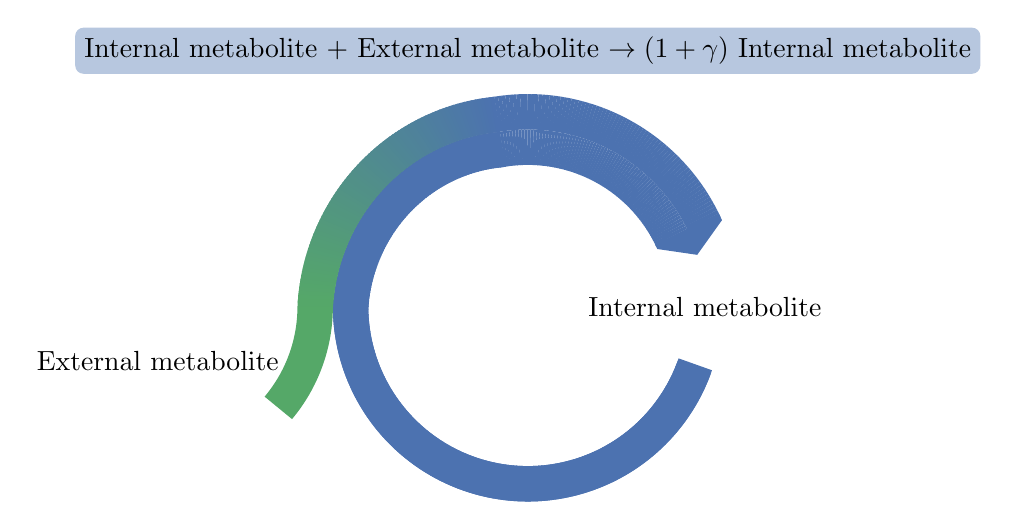
\begin{tikzpicture}
\begin{scope} [shift={(-6.6cm,-4cm)}]
  \colorlet{genext}{assimcol}
  \colorlet{genmed}{blue}
  \colorlet{geninit}{blue}

  \newlength\imrad;
  \newlength\ierad;
  \newlength\esrad;
  \newlength\emrad;
  \newlength\eerad;
  \pgfmathsetlength{\imrad}{\autocatalrad-\blendfrac*\arcwidth};
  \pgfmathsetlength{\ierad}{\autocatalrad-0.5*\arcwidth};
  \pgfmathsetlength{\esrad}{\autocatalrad+\arcwidth};
  \pgfmathsetlength{\emrad}{\autocatalrad+\arcwidth-\blendfrac*\arcwidth};
  \pgfmathsetlength{\eerad}{\autocatalrad+0.5*\arcwidth};

    \shadedarc[\autocatalscale*\arcwidth]{-20}{-180}{\autocatalscale*\autocatalrad}{\autocatalscale*\autocatalrad}{genmed}{geninit};
    \shadedarc[\autocatalscale*\arcwidth]{100}{180}{\autocatalscale*\imrad}{\autocatalscale*\autocatalrad}{genmed}{geninit};
    \shadedarc[\autocatalscale*\arcwidth]{100}{180}{\autocatalscale*\emrad}{\autocatalscale*\esrad}{genext}{geninit};
    \coloredarc[\autocatalscale*\arcwidth]{25}{100}{\autocatalscale*\eerad}{\autocatalscale*\emrad}{genext!0.5!geninit};
    \coloredarc[\autocatalscale*\arcwidth]{25}{100}{\autocatalscale*\ierad}{\autocatalscale*\imrad}{genext!0.5!geninit};

  \fill[genext!0.5!geninit] (\fromang+\deltaang+1:\autocatalscale*\autocatalrad-\autocatalscale*\arcwidth) arc (\fromang+\deltaang+1:\fromang+\deltaang-1:\autocatalscale*\autocatalrad-\autocatalscale*\arcwidth)
       -- (\fromang+\deltaang-1-\protrude:\autocatalscale*\autocatalrad) -- (\fromang+\deltaang-1:\autocatalscale*\autocatalrad+\autocatalscale*\arcwidth) arc (\fromang+\deltaang-1:\fromang+\deltaang+1:\autocatalscale*\autocatalrad+\autocatalscale*\arcwidth)
       -- cycle;

       %% \assimilatedcol input arc
       \draw[color=genext!99.5!geninit,line width=\autocatalscale*\arcwidth] (180:\autocatalscale*\esrad) arc(0:-40:2cm) node [pos=0.5,color=black,left] (ext) {External metabolite};
    \node at (0:\autocatalscale*\autocatalrad) (int) {Internal metabolite};
    \node [rectangle,fill=autocatacyc!40,rounded corners=3pt] at (90:\autocatalscale*\autocatalrad+1cm) (eq) {Internal metabolite + External metabolite $\rightarrow (1+\gamma)$ Internal metabolite};
  \end{scope}
\end{tikzpicture}

}
\caption{
    \label{fig:autocataldef}
  A basic autocatalytic cycle requires an internal metabolite in order to assimilate the external metabolite into the cycle, increasing the amount of the internal metabolite.}
\end{figure}

 
While less than a handful of autocatalytic cycles following this definition are widely known, a systematic search in central carbon metabolism yields several autocatalytic cycles that are not usually considered as such.
We find it useful to group the identified autocatalytic cycles in central carbon metabolism into four classes:
\begin{enumerate}
    \item The glyoxylate cycle within the TCA cycle, that can be used to produce two malate molecules from a single isocitrate molecule, assimilating acetyl-CoA, then converting the two malate molecules with extra acetyl-CoA into two isocitrate molecules \cite{Kornberg1966-lh}.
    \item Glycolysis based cycles using phosphoenolpyruvate (PEP) to transport sugar substrates using the phosphotransferase system (PTS), then converting the imported substrate into two PEP molecules.
    \item Various parts of the pentose-phosphate pathway (PP) assimilating imported sugars that are incorporated into central carbon metabolism as the intermediate metabolites: erythrose-4P, sedoheptulose-7P, ribose-5p or xylulose-5p to later produce these carbon compounds at higher stoichiometries.
    \item Cycles assimilating glycerone-phosphate and using the Entner-Doudoroff (ED) pathway \cite{Entner1952-xs}.
        They first use the fructose bisphosphate aldolase reaction in the reverse direction, producing fructose-1,6-bisphosphate from glyceraldehyde-3-phosphate, then convert the fructose back into two glyceraldehyde-3-phosphate.
\end{enumerate}

We note that the algorithm used in our systematic search is incomplete, meaning additional autocatalytic cycles may exist in central carbon metabolism, as well as in larger metabolic networks.
Further work will enable a more robust algorithm to identify additional autocatalytic cycles in full metabolic networks.

The ubiquity of autocatalytic cycles in central carbon metabolism suggests that unique features of autocatalytic cycles, as derived below, may constrain and shape the kinetic parameters of a broad set of enzymes central to metabolism.

\begin{figure}[h!]
\resizebox{1\linewidth}{!}{
  \begin{tikzpicture}
 \colorlet{ptsinit}{cyan}
  \colorlet{cbbinit}{yellow}
  \colorlet{glyinit}{magenta}

  \pgfmathsetlength{\assimwidth}{1.5pt};

  \node[metaboliteStyle] (g6p) {g6p};

  %%%% upper pts
  \node[shape=coordinate,left=12mm of g6p.center] (ptsmid) {};
  \node[metaboliteStyle,left=7mm of ptsmid,rectangle,draw=assimcol,rounded corners=2pt] (gluc) {gluc};
  \node[metaboliteStyle,shift={(-7mm,-7mm)},gray] at (g6p.center) (pyr1) {pyr};
  \draw[assimcol,line width=\assimwidth] (gluc) -- (ptsmid);
  \draw[->] (ptsmid) [out=0,in=90] to (pyr1);

  \node[metaboliteStyle,below=of g6p.center] (f6p) {f6p};
  \node[metaboliteStyle,below=of f6p] (fbp) {fbp};
  \node[metaboliteStyle,shape=coordinate,below=of fbp.center](fbamid) {};
  \node[metaboliteStyle,below left=of fbamid.center] (dhap) {dhap};
  \node[metaboliteStyle,below right=of fbamid] (gap) {gap};
  \node[metaboliteStyle,below=of gap.center] (bpg) {bpg};
  \node[metaboliteStyle,below=of bpg.center] (3pg) {3pg};
  \node[metaboliteStyle,below=of 3pg.center] (2pg) {2pg};
  \node[metaboliteStyle,below=of 2pg.center] (pep) {pep};
  \node[metaboliteStyle,below=of pep.center] (pyr) {pyr};
  \node[metaboliteStyle,below=of pyr.center,rectangle,draw=assimcol,rounded corners=2pt] (aca) {accoa};
  \node[shape=coordinate,below=of aca] (dummyglta) {};
  \node[metaboliteStyle,left=of dummyglta] (oaa) {oaa};
  \node[metaboliteStyle,right=of dummyglta] (cit) {cit};
  \node[metaboliteStyle,right=of cit] (icit) {icit};
  \node[metaboliteStyle,below=of icit.center] (akg) {akg};
  \node[metaboliteStyle,below=of akg.center] (sca) {sca};
  \node[metaboliteStyle,below=of oaa.center] (mal) {mal};
  \node[metaboliteStyle,below=of mal.center] (fum) {fum};
  \node[metaboliteStyle,right=of mal] (glx) {glx};
  \node[metaboliteStyle,right=of fum] (suc) {suc};
  \node[metaboliteStyle,right=of g6p] (6pgi) {6pgi};
  \node[metaboliteStyle,shape=coordinate,right=of f6p] (s7pspace) {};
  \node[metaboliteStyle,right=of s7pspace] (s7p) {s7p};
  \node[metaboliteStyle,right=of s7p] (r5p) {r5p};
  \node[metaboliteStyle,right=of r5p] (ru5p) {ru5p};
  \node[metaboliteStyle,above=of ru5p.center] (6pgc) {6pgc};
  \node[metaboliteStyle,] at (fbp.center -| s7p.center) (e4p) {e4p};
  \node[metaboliteStyle,] at(e4p.center -| r5p.center) (xu5p) {xu5p};
  \node[metaboliteStyle,] at(3pg.center -| ru5p.center) (rub) {rubp};
  \iftoggle{eddpathway}{
      \node[metaboliteStyle,right=of ru5p] (kdg) {kdg};
      \node[shape=coordinate,] at (fbamid -| kdg.center) (eddtop) {};
      \node[shape=coordinate,] at ([yshift=-0.5mm]gap.center -| xu5p.center) (eddtopbr) {};
      \node[shape=coordinate,] at (2pg.center -| kdg.center) (eddbottom) {};
      \node[shape=coordinate,] at (pyr.center -| rub.center) (eddbottombr) {};
      \draw[->] (6pgc) [out=0,in=90] to (kdg);
      \draw[] (kdg) [out=-90,in=90] to (eddtop);
      \draw[] (eddtop) [out=-90,in=0] to (eddtopbr);
      \draw[->] (eddtopbr) [out=180,in=0] to ([yshift=-0.5mm]gap.east);
      \draw[] (eddtop) [out=-90,in=90] to (eddbottom);
      \draw[] (eddbottom) [out=-90,in=0] to (eddbottombr);
      \draw[->] (eddbottombr) [out=180,in=0] to (pyr.east);
    }{ }
  \node[metaboliteStyle,rectangle,draw=assimcol,rounded corners=2pt] at(2pg -| xu5p.center) (co2) {\ce{CO2}};
  \draw[->] (g6p) -- (f6p);
  \draw[->] ([xshift=0.1cm]f6p.south) -- ([xshift=0.1cm]fbp.north);
  \draw[<-] ([xshift=-0.1cm]f6p.south) -- ([xshift=-0.1cm]fbp.north);
  \draw [<-] (fbp) [out=-90,in=90] to (fbamid);
  \draw [->] (fbamid) [out=-90,in=45] to (dhap);
  \draw [->] (fbamid) [out=-90,in=135] to (gap);
  \draw [<->] (dhap) -- (gap);
  \draw[<->] (gap) -- (bpg);
  \draw[<->] (bpg) -- (3pg);
  \draw[->] (3pg) -- (2pg);
  \draw[->] (2pg) -- (pep);
  \draw[->] (pep) -- (pyr);
  \draw[->] (pyr) -- (aca);
  \draw[->] (oaa) -- (cit) node [pos=0.9] (midglta) {};
  \draw [assimcol,line width=\assimwidth] (aca) [out=-70,in=180] to (midglta);
  \draw[->] (cit) -- (icit);
  \draw[->] (icit) -- (suc) node [pos=0.3] (midacea) {};
  \draw[->] (midacea) [out=220,in=0] to (glx);
  \draw[->] (icit) -- (akg);
  \draw[->] (akg) -- (sca);
  \draw[->] (sca) -- (suc);
  \draw[->] (suc) -- (fum);
  \draw[->] (fum) -- (mal);
  \draw[->] (glx) -- (mal) node [pos=0.9] (midaceb) {};
  \draw[->] (mal) -- (oaa);
  \draw[assimcol,line width=\assimwidth] (aca) [out=-90,in=0] to (midaceb);
  \draw[->] (g6p) -- (6pgi);
  \draw[->] (6pgi) -- (6pgc);
  \draw[->] (6pgc) -- (ru5p);
  \draw[<-] (ru5p) -- (xu5p);
  \draw[<-] (ru5p) -- (r5p);
  \path[] (r5p) -- (gap) coordinate [pos=0.2] (midtkt1) {};
  \draw[<-] (xu5p) [out=180,in=-90] to (midtkt1);
  \draw[] (midtkt1) [out=90,in=0] to (s7p);
  \draw[<-] (r5p) [out=180,in=90] to (midtkt1);
  \draw[] (midtkt1) [out=270,in=0] to (gap);
  \path[] (e4p) -- (gap) coordinate [pos=0.4] (midtkt2) {};
  \draw[<-] (e4p) [out=-60,in=0] to (midtkt2);
  \draw[] (midtkt2) [out=180,in=90] to (gap);
  \draw[<-] (xu5p) [out=245,in=0] to (midtkt2);
  \draw[] (midtkt2) [out=180,in=-30] to (f6p);
  \path[] (e4p) -- (s7pspace) coordinate [pos=0.5] (midtal) {};
  \draw[] (midtal) [out=90,in=0] to (f6p);
  \draw[<-] (s7p) [out=180,in=90] to (midtal);
  \draw[] (midtal) [out=-90,in=180] to (e4p);
  \draw[<-] (gap) [out=55,in=-90] to (midtal);
  \node[shape=coordinate,left=2.5cm of pep.center] (pts3) {};
  \draw[] (pep) [out=180,in=0] to (pts3);
  \node[shape=coordinate,left=2.5cm of pyr.center] (pts5) {};
  \node[shape=coordinate,left=2.1cm of f6p.center] (ptstop) {};
  \node[shape=coordinate] at(ptstop |- 2pg.center) (ptsbottom) {};
  \draw[] (pts3) [in=-90,out=180] to (ptsbottom);
  \draw[] (ptsbottom) [in=-90,out=90] to (ptstop);
  \draw[] (ptstop) [in=180,out=90] to (ptsmid);
  \draw[->] (ptsmid) -- (g6p);
  \draw[->] (ru5p) [out=-90,in=90] to (rub);
  \draw[->] (rub) -- (3pg) coordinate [pos=0.9] (rubisco); 
  \draw[assimcol,line width=\assimwidth] (co2) [out=90,in=0] to (rubisco);
  \node[shape=coordinate,shift={(-\highlightrad,-\highlightrad)}] at (pep.south -| ptsbottom) (ptsbottomlimit) {};
  \node[shape=coordinate,shift={(-\highlightrad,\highlightrad)}] at (g6p.north -| ptstop) (ptstoplimit) {};

  \draw[opacity=0.2,fill=ptsinit,rounded corners=\highlightrad,visible on=<3->] ([shift={(\highlightrad,\highlightrad)}]g6p.north east) -- ([xshift=\highlightrad] fbp.east) -- ([shift={(\highlightrad,\highlightrad)}]gap.north east)--([shift={(\highlightrad,-\highlightrad)}]pep.south east) -- (ptsbottomlimit) -- node[midway] (ptsshademid) {} ([yshift=-1.2cm]ptstoplimit) -- ([shift={(-1mm,\highlightrad)}]g6p.north -| ptsmid) -- cycle;

  \draw[very thick,dashed,cyan,->,visible on=<3->] (ptsshademid) -- ++(-1.5cm,0cm); 

  \draw[opacity=0.2,fill=glyinit,rounded corners=\highlightrad,visible on=<4->] ([shift={(-\highlightrad,2*\highlightrad)}]oaa.west) -- ([shift={(\highlightrad,2*\highlightrad)}]icit.east) -- node[midway] (glyshadedmid) {}([shift={(\highlightrad,-0.5*\highlightrad)}]icit.south east) -- ([shift={(0.5*\highlightrad,-2*\highlightrad)}]suc.east) -- ([shift={(-\highlightrad,-2*\highlightrad)}]fum.west) -- cycle;

  \draw[very thick,dashed,magenta,->,visible on=<4->] (glyshadedmid) -- ++(1.5cm,0cm); 

  \node[shape=coordinate] at (dhap.south -| gap.west) (cbbmid) {};
  \draw[opacity=0.2,fill=cbbinit,rounded corners=\highlightrad,visible on=<2->] ([shift={(-\highlightrad,2.2*\highlightrad)}]f6p.west) -- ([shift={(3*\highlightrad,2.2*\highlightrad)}]ru5p.center) -- node[midway] (cbbshadedmid) {} ([shift={(3*\highlightrad,-2*\highlightrad)}]rub.center) -- ([shift={(-\highlightrad,-2*\highlightrad)}]3pg.west) -- ([shift={(-\highlightrad,-\highlightrad)}]cbbmid) -- ([shift={(-0.5*\highlightrad,-\highlightrad)}]dhap.south west) -- ([shift={(-0.5*\highlightrad,0.5*\highlightrad)}]dhap.north west) -- ([xshift=-\highlightrad]fbp.west) -- cycle;

  \draw[very thick,dashed,cbbinit,->,visible on=<2->] (cbbshadedmid) -- ++(1.5cm,0cm); 

  %% CBB cycle
  \begin{scope} [shift={(11.3cm,-4.5cm)},radius=2cm,visible on=<2->]
    \draw[lightgray,rounded corners=\highlightrad] (-2.7,-2.1) rectangle +(4.6,4.5);

    \iftoggle{article} {
        \node at (-2.2cm,2cm) (I) {\large  \textbf{I}};
    }{ }
    \node[anchor=north] at(-0.4cm,-2.2cm) (cbbreac) {{\fontfamily{cmss}\selectfont 5}  3pg + {\fontfamily{cmss}\selectfont 3} \ce{CO2} $\rightarrow$ {\fontfamily{cmss}\selectfont 6} 3pg};
    \colorlet{cbbmed}{blue}
    \colorlet{cbbext}{assimcol}
  

    \pgfmathsetlength{\cbbwidth}{\arcwidth*0.2};
    \pgfmathsetlength{\cbbtotwidth}{\cbbwidth+\arcwidth};
    \pgfmathsetlength{\cbbimrad}{\autocatalrad-\blendfrac*0.5*\cbbtotwidth};
    \pgfmathsetlength{\cbbierad}{\autocatalrad-0.5*\cbbwidth};
    \pgfmathsetlength{\cbbesrad}{\autocatalrad+0.5*\cbbtotwidth};
    \pgfmathsetlength{\cbbemrad}{\autocatalrad+0.5*\cbbtotwidth-\blendfrac*0.5*\cbbtotwidth};
    \pgfmathsetlength{\cbbeerad}{\autocatalrad+0.5*\arcwidth};

    \shadedarc{-20}{-180}{\autocatalrad}{\autocatalrad}{cbbmed}{cbbinit};
    \shadedarc{100}{180}{\cbbimrad}{\autocatalrad}{cbbmed}{cbbinit};
    \coloredarc{25}{100}{\cbbierad}{\cbbimrad}{cbbinit};
    \shadedarc[\cbbwidth]{100}{180}{\cbbemrad}{\cbbesrad}{cbbext}{cbbinit};
    \coloredarc[\cbbwidth]{25}{100}{\cbbeerad}{\cbbemrad}{cbbinit};

%% \assimilatedcol input arc
        \draw[color=cbbext,line width=\cbbwidth]
        (\fromang:\autocatalrad+0.5*\arcwidth+0.5*\cbbwidth)
        arc (0:\inputang:2cm)
        node [pos=0.5,color=black,anchor=east] (co2c) {\ce{CO2}};
%% arrowhead
    \fill[cbbinit]
      (\fromang+\deltaang+1:\autocatalrad-0.5*\arcwidth-0.5*\cbbwidth)
      arc (\fromang+\deltaang+1:\fromang+\deltaang-1:\autocatalrad-0.5*\arcwidth-0.5*\cbbwidth)
      -- (\fromang+\deltaang-1-\protrude:\autocatalrad)
      -- (\fromang+\deltaang-1:\autocatalrad+0.5*\arcwidth+0.5*\cbbwidth)
      arc (\fromang+\deltaang-1:\fromang+\deltaang+1:\autocatalrad+0.5*\arcwidth+0.5*\cbbwidth)
      -- cycle;

%% metabolites
        \node at (0:\autocatalrad) (3pgc) {3pg};
        \node at (220:\autocatalrad-4.7mm) (rubc) {rubp};

  \end{scope}

  %glyoxilate cycle
\begin{scope} [shift={(9cm,-13.5cm)},radius=2cm,visible on=<4->]
  \draw[lightgray,rounded corners=\highlightrad] (-2.4cm,-2.6cm) rectangle +(4.5,5.1);

  \iftoggle{article} {
      \node at (-2cm,2.2cm) (II) {\large  \textbf {II}};
  }{ }

  \node[anchor=north] at(-0.15cm,-2.7cm) (glyreac) {mal + {\fontfamily{cmss}\selectfont 2} accoa $\rightarrow$ {\fontfamily{cmss}\selectfont 2} mal};
  \colorlet{glymed}{blue}
  \colorlet{glyext}{assimcol}
  \colorlet{glyinter}{blue}
  
    \pgfmathsetlength{\glywidth}{\arcwidth*0.5};
    \pgfmathsetlength{\glytotwidth}{\glywidth+\arcwidth};
    \pgfmathsetlength{\glyfinwidth}{\glytotwidth+\glywidth};
    \pgfmathsetlength{\glyimrad}{\autocatalrad-\blendfrac*0.5*\glywidth};
    \pgfmathsetlength{\glyimmrad}{\autocatalrad-0.5*\glywidth};
    \pgfmathsetlength{\glyemmrad}{\glyimmrad+0.5*\glytotwidth};
    \pgfmathsetlength{\glyemmmrad}{\glyemmrad+0.5*\glywidth};
    \pgfmathsetlength{\glyeamrad}{\autocatalrad+0.5*\glytotwidth};
    \pgfmathsetlength{\glyierad}{\autocatalrad-0.5*\glywidth};
    \pgfmathsetlength{\glyesrad}{\autocatalrad+0.5*\glytotwidth};
    \pgfmathsetlength{\glyemrad}{\autocatalrad+0.5*\glyfinwidth-\blendfrac*0.5*\glywidth};
    \pgfmathsetlength{\glyeerad}{\autocatalrad+0.5*\glytotwidth};

    \shadedarc{-20}{-90}{\autocatalrad}{\autocatalrad}{glymed}{glyinit};
    \shadedarc{-150}{-90}{\glyimmrad}{\autocatalrad}{glymed}{glyinter};
    \shadedarc[\glywidth]{-150}{-90}{\glyemmrad}{\glyeamrad}{glyext}{glyinter};

    \draw[color=glyext,line width=\glywidth] (-90:\autocatalrad+0.5*\glytotwidth) arc(90:50:2cm) node [pos=0.5,color=black,anchor=north,xshift=-1.5mm] (acac) {accoa};

    \coloredarc[\glytotwidth]{160}{90}{\glyimmrad}{\glyimmrad}{glyinter};

    \draw[color=glyext,line width=\glywidth] (90:\glyemmmrad) arc(-90:-130:2cm) node [pos=0.5,color=black,anchor=south,xshift=2mm] (acac) {accoa};

    \shadedarc[\glytotwidth]{50}{90}{\glyimrad}{\glyimmrad}{glyinter}{glyinit};
    \coloredarc[\glytotwidth]{50}{25}{\glyimrad}{\glyierad}{glyinit};

    \shadedarc[\glywidth]{90}{50}{\glyemmmrad}{\glyemrad}{glyinit}{glyext};
    \coloredarc[\glywidth]{50}{25}{\glyemrad}{\glyeerad}{glyinit};


    \node at (0:\autocatalrad) (malc) {mal};
    \node at (180:\autocatalrad) (glxc) {glx+fum};
    \node at (-50:\autocatalrad-4.5mm) (oaa) {oaa};

  \fill[glyinit] (\fromang+\deltaang+1:\autocatalrad-\arcwidth) arc (\fromang+\deltaang+1:\fromang+\deltaang-1:\autocatalrad-\arcwidth)
       -- (\fromang+\deltaang-1-\protrude:\autocatalrad) -- (\fromang+\deltaang-1:\autocatalrad+\arcwidth) arc (\fromang+\deltaang-1:\fromang+\deltaang+1:\autocatalrad+\arcwidth)
       -- cycle;

  \fill[glyinter] (-149:\autocatalrad-\arcwidth+0.5*\glywidth) arc (-149:-161:\autocatalrad-\arcwidth+0.5*\glywidth)
       -- (-161-\protrude:\autocatalrad) -- (-161:\autocatalrad+\arcwidth-0.5*\glywidth) arc (-161:-149:\autocatalrad+\arcwidth-0.5*\glywidth)
       -- cycle;
  \end{scope}


  %pts cycle
\begin{scope} [shift={(-5.8cm,-5.5cm)},radius=2cm,visible on=<3->]
  \draw[lightgray,rounded corners=\highlightrad] (-2.5,-3) rectangle +(4.5,5.5);

  \iftoggle{article} {
      \node at (-2cm,2.2cm) (III) {\large  \textbf {III}};
  }{ }

  \node[anchor=north] at(-0.25cm,-3.1cm) (ptsreac) {pep + gluc $\rightarrow$ {\fontfamily{cmss}\selectfont 2} pep + pyr};
    \colorlet{ptsmed}{blue}
    \colorlet{ptsext}{assimcol}

    \pgfmathsetlength{\ptsierad}{\autocatalrad*0.5};
    \pgfmathsetlength{\ptsimrad}{\autocatalrad-0.5*\arcwidth};
    \pgfmathsetlength{\ptsarcwidth}{2*\arcwidth};
    \pgfmathsetlength{\ptsesrad}{\autocatalrad+0.5*\arcwidth+0.5*\ptsarcwidth};
    \pgfmathsetlength{\ptsemrad}{\autocatalrad+0.5*\ptsarcwidth};

    \shadedarc{-20}{-120}{\autocatalrad}{\autocatalrad}{ptsmed}{ptsinit};
    \shadedarc{160}{240}{\ptsimrad}{\autocatalrad}{ptsmed}{ptsinit};
    \shadedarc{70}{160}{\ptsierad}{\ptsimrad}{ptsinit}{white};
    \shadedarc[\ptsarcwidth]{160}{240}{\ptsemrad}{\ptsesrad}{ptsext}{ptsinit};
    \coloredarc[\ptsarcwidth]{25}{160}{\autocatalrad}{\ptsemrad}{ptsinit};

  \fill[ptsinit] (\fromang+\deltaang+1:\autocatalrad-\arcwidth) arc (\fromang+\deltaang+1:\fromang+\deltaang-1:\autocatalrad-\arcwidth)
       -- (\fromang+\deltaang-1-\protrude:\autocatalrad) -- (\fromang+\deltaang-1:\autocatalrad+\arcwidth) arc (\fromang+\deltaang-1:\fromang+\deltaang+1:\autocatalrad+\arcwidth)
       -- cycle;

       %% \assimilatedcol input arc
       \draw[color=ptsext,line width=\ptsarcwidth] (240:\ptsesrad) arc(60:20:2cm) node [pos=0.5,color=black,left,shift={(-1mm,-2mm)}] (glucc) {gluc};
    \node at (0:\autocatalrad) (pepc) {pep};
    \node at (70:\ptsierad) (pyrc) {pyr};
  \end{scope}


\end{tikzpicture}


}
\caption{
    \label{fig:realautocatal}
Three representative autocatalytic cycles in central carbon metabolism: (I) The Calvin-Benson-Bassham cycle; (II) The glyoxylate cycle; (III) A cycle using the PTS system to assimilate glucose.
}
\end{figure}

\subsection{Steady state existence and stability analysis of a simple autocatalytic cycle}
To explore general principles governing the dynamic behavior of autocatalytic cycles, we consider the simple autocatalytic cycle depicted in Figure \ref{fig:simplecycle}A.
This cycle has a single intermediate metabolite, $X$.
We denote the flux through the autocatalytic reaction of the cycle by $f_a$, such that for any unit of $X$ consumed, it produces two units of $X$.
The autocatalytic reaction obviously consumes some external metabolite, which we assume to be at a constant concentration.
We denote the flux through the reaction branching out of the cycle by $f_b$.
    We assume simple, irreversible Michaelis-Menten kinetics for the two reactions such that:
    \begin{eqnarray*}
      f_a = \frac{V_{\max,a}X}{K_{M,a}+X} \\
      f_b = \frac{V_{\max,b}X}{K_{M,b}+X}
    \end{eqnarray*}
    where all the kinetic parameters are positive.
    Using these simple forms allows both an analytic solution to be obtained and a didactic presentation.
    We discuss more general cases below.
    \begin{figure}[h!]
        \begin{tikzpicture}[>=latex',node distance = 2cm]
    \tikzset{
        vstyle/.style={opacity=0.3,pattern=north west lines,cyan,visible on=<6->}}
    \tikzset{
        kstyle/.style={opacity=0.3,pattern=north east lines,magenta,visible on=<6->}}
  \begin{scope}[shift={(-4cm,4cm)}]
        \node at (0:1cm) (X) {$X$};
        \node[shape=coordinate] (orig) {};
        \draw [->,line width=1pt,autocatacyc] (X.south) arc (345:15:1cm) node [pos=0.75,above] (fa) {$f_a:$\small{$E+X\rightarrow2X$}} node [pos=0.5,shape=coordinate] (midauto) {};
        \draw [line width=1pt,assimcol] (midauto) arc (0:-40:1cm) node [pos=1,left] (e) {$E$};
        \draw [->,line width=1pt,branchout] ([xshift=1mm]X.south) arc (190:270:1cm) node [pos=0.3,right] {$f_b$};
        \iftoggle{article} {
            \node at (-2.4cm,1.3cm) (A) {(A)};
        }{}
        \begin{customlegend}[legend entries={$f_a$,$V_{\max,b}>V_{\max,a}$,$f_b$,$\sfrac{V_{\max,b}}{V_{\max,a}}<\sfrac{K_{M,b}}{K_{M,a}}$,$\dot{X}=f_a-f_b$},legend style={right=2.5cm of orig,anchor=west,name=legend1,visible on=<3->},legend columns=2]
          \addlegendimage{autocatacyc,fill=black!50!red,sharp plot,line width=1pt}
          \addlegendimage{vstyle,area legend,visible on=<4->}
          \addlegendimage{branchout,fill=black!50!red,sharp plot,line width=1pt}
          \addlegendimage{kstyle,area legend,visible on=<4->}
          \addlegendimage{sumcolor,fill=black!50!red,sharp plot,dashed,line width=1pt}
        \end{customlegend}
  \end{scope}
  \begin{scope}[shift={(-1.5cm,-\gridsize/2)}]
    \begin{axis}[name=phase,clip=false,xmin=0,ymin=0,xmax=2,ymax=2,ylabel={\Large{$\sfrac{V_{\max,b}}{V_{\max,a}}$}},xlabel={\Large{$\sfrac{K_{M,b}}{K_{M,a}}$}},samples=6,width=\gridsize,height=\gridsize,ytick={0,1,2},xtick={0,1,2},visible on=<6->]
        \addplot[domain=0:2,dotted,black,thick] {x};
        \addplot[dotted,black,thick] coordinates {(0,1) (2,1)};
        \draw[kstyle] (axis cs:0,0) -- (axis cs:2,2) -- (axis cs:2,0) --cycle;
        \draw[vstyle] (axis cs:0,1) -- (axis cs:2,1) -- (axis cs:2,2) -- (axis cs:0,2) --cycle;
        \draw[->,black!50,dashed] (axis cs:0.25,1.4) -- +(-1.9cm,0cm);
        \draw[->,black!50,dashed] (axis cs:1.75,1.4) -- +(1.1cm,0cm);
        \draw[->,black!50,dashed] (axis cs:0.25,0.6) -- +(-1.9cm,0cm);
        \draw[->,black!50,dashed] (axis cs:1.75,0.6) -- +(1.1cm,0cm);
        \node[align=left,anchor=east] at (axis cs:1.75,1.4) (I) {I};
        \node[align=right,anchor=west] at (axis cs:0.25,1.4) (II) {II};
        \node[align=right,anchor=west] at (axis cs:0.25,0.6) (III) {III};
        \node[align=left,anchor=east] at (axis cs:1.75,0.6) (IV) {IV};
      \end{axis}

\iftoggle{article} {
        \pgfmathsetlength{\plotwidthanim}{\plotwidth}
        \pgfmathsetlength{\plotheightanim}{\plotheight}
        \pgfmathsetlength{\plotshift}{1mm}
}{
    \only<4-> {
        \pgfmathsetlength{\plotwidthanim}{\plotwidth}
        \pgfmathsetlength{\plotheightanim}{\plotheight}
        \pgfmathsetlength{\plotshift}{1mm}
    }
}

      \begin{axis}[name=plot1,axis x line=middle,axis y line=left,xlabel near ticks,ylabel near ticks,xmin=0,ymin=-2.5,xmax=2.9,ymax=5.9,xlabel={[$X$]},ylabel={flux},samples=60,width=\plotwidthanim,height=\plotheightanim,clip=false,yticklabels={,,},xticklabels={,,},tick label style={major tick length=0pt},at=(phase.right of north east),anchor=left of north west,ylabel style={name=ylabel1},xshift=\plotshift,visible on=<2->]%,axis background/.style={fill=cyan!50!magenta,opacity=0.3}]
        \addplot[domain=0:2.9,autocatacyc,thick] {3*x/(0.1+x)};
        \addplot[domain=0:2.9,branchout,thick] {5*x/(1+x)};
        \addplot[domain=0:2.9,sumcolor,thick,dashed,visible on=<3->] {3*x/(0.1+x)-5*x/(1+x)};
        \addplot[dashed,gray,thick] coordinates {(1.25,0) (1.25,2.77)};
        \node[right,align=left,visible on=<5->] (onetext) at (axis cs:0.05,4.7) {\scriptsize stable non-zero\\[-0.4em]\scriptsize steady state};
      \end{axis}
      \node[draw,fit=(plot1) (ylabel1),line width=2pt, fill=none,rounded corners=3pt,cyan!50!magenta,opacity=0.6,visible on=<6->]{};

      \begin{axis}[name=plot2,axis x line=middle,axis y line=left,xlabel near ticks,ylabel near ticks,xmin=0,ymin=-2.5,xmax=2.9,ymax=5.9,xlabel={[$X$]},ylabel={flux},samples=60,at=(phase.left of north west),anchor=right of north east,width=\plotwidth,height=\plotheight,yticklabels={,,},xticklabels={,,},tick label style={major tick length=0pt},ylabel style={name=ylabel2},xshift=-1mm,visible on=<4->]%,axis background/.style=vstyle]
        \addplot[domain=0:4,autocatacyc,thick] {4*x/(1+x)};
        \addplot[domain=0:4,branchout,thick] {5*x/(0.2+x)};
        \addplot[domain=0:4,sumcolor,thick,dashed,visible on=<5->] {4*x/(1+x)-5*x/(0.2+x)};
        \node[right,align=left,visible on=<5->] (twotext) at (axis cs:0.0,5) {\scriptsize stable zero steady state};
      \end{axis}
      \node[draw,fit=(plot2) (ylabel2),line width=2pt, vstyle,fill=none,rounded corners=3pt]{};

      \begin{axis}[name=plot3,axis x line=middle,axis y line=left,xlabel near ticks,ylabel near ticks,xmin=0,ymin=-2.5,xmax=2.9,ymax=5.9,xlabel={[$X$]},ylabel={flux},samples=60,width=\plotwidth,height=\plotheight,yticklabels={,,},xticklabels={,,},tick label style={major tick length=0pt},at=(phase.left of south west),anchor=right of south east,ylabel style={name=ylabel3},xshift=-1mm,visible on=<4->]
        \addplot[domain=0:4,autocatacyc,thick] {5*x/(1+x)};
        \addplot[domain=0:4,branchout,thick] {3*x/(0.1+x)};
        \addplot[domain=0:4,sumcolor,thick,dashed,visible on=<5->] {5*x/(1+x)-3*x/(0.1+x)};
        \addplot[dashed,gray,thick] coordinates {(1.25,0) (1.25,2.77)};
        \node[right,align=left,visible on=<5->] (threetext) at (axis cs:0.05,4.7) {\scriptsize unstable non-zero\\[-0.4em]\scriptsize steady state};
      \end{axis}
      \node[draw,fit=(plot3) (ylabel3),line width=2pt, fill=none,rounded corners=3pt,opacity=0.2, black!40,visible on=<6->]{};

      \begin{axis}[name=plot4,axis x line=middle,axis y line=left,xlabel near ticks,ylabel near ticks,xmin=0,ymin=-2.5,xmax=2.9,ymax=5.9,xlabel={[$X$]},ylabel={flux},samples=60,at=(phase.right of south east),anchor=left of south west,width=\plotwidth,height=\plotheight,yticklabels={,,},xticklabels={,,},tick label style={major tick length=0pt},ylabel style={name=ylabel4},xshift=1mm,visible on=<4->]%,axis background/.style=kstyle]
        \addplot[domain=0:2.9,autocatacyc,thick] {5*x/(0.2+x)};
        \addplot[domain=0:2.9,branchout,thick] {4*x/(1+x)};
        \addplot[domain=0:2.9,sumcolor,thick,dashed,visible on=<5->] {5*x/(0.2+x)-4*x/(1+x)};
        \node[right,align=left,visible on=<5->] (fourtext) at (axis cs:0.05,5) {\scriptsize  no stable steady state};
     \end{axis}
      \node[draw,fit=(plot4) (ylabel4),line width=2pt, kstyle,fill=none,rounded corners=3pt]{};

        \iftoggle{article} {
          \node [at=(plot2.north west),xshift=-0.6cm,yshift=0.35cm] (B) {(B)};
        }{}
    \end{scope}
  \end{tikzpicture}


      \caption{\label{fig:simplecycle}
        (A) A simple autocatalytic cycle induces two fluxes, $f_a$ and $f_b$ as a function of the concentration of $X$.
        These fluxes follow simple Michaelis Menten kinetics.
        A steady state occurs when $f_a=f_b$, implying that $\dot{X}=0$.
        The cycle always has a steady state at $X=0$.
        The slope of each reaction at $X=0$ is $\sfrac{V_{\max}}{K_m}$.
        A steady state is stable if at the steady state concentration $\frac{d\dot{X}}{dX}<0$.
        (B) Each set of kinetic parameters, $V_{\max,a},V_{\max,b},K_{M,a},K_{M,b}$ determines two characteristics of the system: 
        If $V_{\max,b}>V_{\max,a}$, then a stable steady state concentration must exist as for high concentrations of $X$ the branching reaction will reduce its concentration (cyan domain, cases (I) and (II)).
        If $\sfrac{V_{\max,b}}{K_{M,b}}<\sfrac{V_{\max,a}}{K_{M,a}}$, implying that $\sfrac{V_{\max,b}}{V_{\max,a}}<\sfrac{K_{M,b}}{K_{M,a}}$, then zero is a non-stable steady state concentration as if $X$ is slightly higher than zero, the autocatalytic reaction will carry higher flux, further increasing the concentration of $X$ (magenta domain, cases (I) and (IV)).
    At the intersection of these two domains a non-zero, stable steady state concentration exists (I).}
    \end{figure}

    We characterize the metabolic state of this system by the concentration of the metabolite $X$.
    We note that knowing the concentration of $X$ suffices in order to calculate the fluxes originating from it, $f_a$ and $f_b$, thus fully defining the state of the system.
    A steady state of the system is defined as a concentration, $X^*$, which induces fluxes that keep the concentration steady, such that the total in-flux to $X$ is exactly equal to the total out-flux from it.
    In our example, the outgoing flux from $X$ is $f_a+f_b$ and the incoming flux to $X$ is $2f_a$, so at steady state it holds that:
    \begin{equation}
      \label{eq:xdyna}
      \dot X = \frac{dX}{dt} = 2f_a - (f_a + f_b) = 0
    \end{equation}

    Expanding this condition we get:
    \begin{equation*}
      \dot X = 0 \Rightarrow f_a = f_b \Rightarrow \frac{V_{\max,a}X}{K_{M,a}+X}=\frac{V_{\max,b}X}{K_{M,b}+X}
    \end{equation*}
    which is satisfied either if $X=0$ or if:
    \begin{equation}
      \label{eq:xstst}
      X=\frac{V_{\max,b}K_{M,a}-V_{\max,a}K_{M,b}}{V_{\max,a}-V_{\max,b}}
    \end{equation}
    The concentration of $X$ cannot be negative, and thus we get a constraint on the kinetic parameters for which a positive steady state exists:
    \begin{equation*}
      \frac{V_{\max,b}K_{M,a}-V_{\max,a}K_{M,b}}{V_{\max,a}-V_{\max,b}}>0 \Rightarrow \frac{\frac{V_{\max,b}}{K_{M,b}}-\frac{V_{\max,a}}{K_{M,a}}}{V_{\max,a}-V_{\max,b}}>0
    \end{equation*}
    In order to gain intuition for this relationship we note that $\frac{V_{\max}}{K_m}$ is the slope of the Michaelis Menten function at $X=0$.
    The constraint states that if $V_{\max,b}<V_{\max,a}$ then it must be that $\frac{V_{\max,b}}{K_{M,b}}>\frac{V_{\max,a}}{K_{M,a}}$ and that if $V_{\max,b}>V_{\max,a}$ then $\frac{V_{\max,b}}{K_{M,b}}<\frac{V_{\max,a}}{K_{M,a}}$.
    The constraint therefore implies that in order for a positive steady state to exist, the reaction with higher maximal flux must have a shallower slope at $X=0$.
    This condition can be intuitively understood, as the reaction with shallower slope at $X=0$ has smaller fluxes for small values of $X$, compared with the other reaction, so unless it has higher fluxes than the other reaction for large values of $X$ (meaning that its maximal flux is higher), the two will not intersect.
    This constraint is graphically illustrated in Figure \ref{fig:simplecycle}B, cases (I) and (III).

    While having a positive concentration steady state is an essential condition to sustain flux, it is not sufficient.
    The positive concentration steady state must also be stable to small perturbations.
    Stability with respect to small perturbations is determined by the response of the system to small deviations from the steady state, $X^*$.
    Mathematically, stability dictates that at $X=X^*$ it holds that $\frac{d\dot X}{dX} <0$, as this  implies that upon a small deviation from the steady state: $X = X^*+\Delta X$ the net flux $\dot X$ will oppose the direction of the deviation.
    If $\Delta X$ is positive then $\dot X$ will be negative at $X^*+\Delta X$, reducing $X$ back to $X^*$, and if $\Delta X$ is negative, $\dot X$ will be positive, increasing $X$ back to $X^*$.

    For the simple kinetics we chose the stability condition requires that:
    \begin{equation}
        \label{eq:stable}
      \frac{d\dot X}{dX}\Big\vert_{X^*} = \frac{V_{\max,a}K_{M,a}}{(K_{M,a}+X^*)^2}-\frac{V_{\max,b}K_{M,b}}{(K_{M,b}+X^*)^2}<0
    \end{equation}
    The analysis is straightforward for the case of $X^*=0$, yielding that $0$ is a stable steady state concentration if $\frac{V_{\max,b}}{K_{M,b}}>\frac{V_{\max,a}}{K_{M,a}}$, corresponding to the area above the diagonal in figure \ref{fig:simplecycle}B, where $\frac{V_{\max,b}}{V_{\max,a}}>\frac{K_{M,b}}{K_{M,a}}$, resulting in cases (II) and (III), and is unstable otherwise.
    The criteria that is of interest, however, is the criteria for stability of the non-zero steady state, $X^*=\frac{V_{\max,b}K_{M,a}-V_{\max,a}K_{M,b}}{V_{\max,a}-V_{\max,b}}$.
    In this case, substituting $X^*$ in equation \ref{eq:stable} gives the opposite condition to that of $X^*=0$, namely that it is stable if $\frac{V_{\max,b}}{K_{M,b}}<\frac{V_{\max,a}}{K_{M,a}}$, corresponding to the magenta domain in figure \ref{fig:simplecycle}B, containing cases (I) and (IV), and unstable otherwise.

    The stability criteria can be generally stated in metabolic control terms \cite{Fell1997-bp} using the notion of elasticity coefficients of reactions, defined as:
    \begin{equation*}
    \varepsilon^f_X=\frac{\partial f}{\partial X}\frac{X}{f}
    \end{equation*}
    In these terms, stability is obtained if and only if the elasticity of the biomass reaction at the positive steady state concentration is greater than the elasticity of the autocatalytic reaction:
    \begin{equation*}
        \frac{df_b}{dX}\Big\vert_{X^*}>\frac{df_a}{dX}\Big\vert_{X^*} \Rightarrow \varepsilon^{f_b}_X>\varepsilon^{f_a}_X
    \end{equation*}
    Using the notion of elasticities will prove useful in the extension of our conclusions to more complex cycles below.
    
    The complete analysis is summed up in Figure \ref{fig:simplecycle}B.
    Domain (I) is the only domain where a positive, stable steady state exists.
    Domains (I) and (III) are the domains at which a positive steady state concentration exists, but in domain (III) that steady state is not stable.
    The domains below the diagonal (cases (I) and (IV)) are the domains where $X^*=0$ is an unstable steady state concentration, so that if another steady state exists, it is stable, but in domain (IV) no positive steady state exists.
    The domains above the diagonal (cases (II) and (III)) are the domains where $X^*=0$ is a stable steady state concentration, so that the other steady state, if it exists, is unstable.

    To conclude, for this simple cycle, we get that in order for a positive-concentration stable steady state to exist (case (I)), two conditions must be satisfied:
    \begin{equation}
    \label{eq:stabconds}
    \begin{dcases}
      & V_{\max,b}>V_{\max,a} \\
      & \frac{V_{\max,b}}{K_{M,b}}<\frac{V_{\max,a}}{K_{M,a}}
    \end{dcases}
    \end{equation}
    meaning that the potential of the biomass generating flux is higher than the autocatalytic flux, ensuring stability, and that at low concentrations of $X$, the autocatalytic reaction starts higher than the biomass generating reaction (as can be inferred from the slopes), ensuring that the two fluxes will be equal for some positive concentration of $X$.

    Interestingly, these conditions imply that if $K_{M,b}<K_{M,a}$ then no positive stable steady state can be achieved, even when allowing changes to the expression levels of the enzymes catalyzing $f_a$ and $f_b$, which only affect $V_{\max,a}$ and $V_{\max,b}$.
    This indicates that stability of autocatalytic cycles depends on inherent kinetic properties of the enzymes involved and cannot always be achieved by modulating expression levels, a conclusion that may be critical in metabolic engineering context.
\subsection{Extensions of the simple autocatalytic cycle model}
    \subsubsection{Generalizing for different autocatalytic stoichiometries}
    Our initial analysis considered an autocatalytic reaction with $1:2$ stoichiometry, such that for every substrate molecule consumed, two are produced.
    Real-world autocatalytic cycles may have different stoichiometries.
    For example, the CBB cycle has a stoichiometry of $5:6$ so that for every 5 molecules of 5-carbon sugars that the autocatalytic reaction consumes, 6 5-carbon sugars are produced.
    We can generalize our analysis by defining $\gamma$ such that for every molecule of $X$ that $f_a$ consumes, it produces $1+\gamma$ molecules of $X$, where $\gamma$ may be a fraction.
    This extension implies that equation \eqref{eq:xdyna} becomes:

    \begin{equation*}
      \dot X = \frac{dX}{dt} = (1+\gamma)f_a - (f_a + f_b) = 0 \Rightarrow \gamma f_a = f_b \Rightarrow \frac{\gamma V_{\max,a}X}{K_{M,a}+X}=\frac{V_{\max,b}X}{K_{M,b}+X}
    \end{equation*}

    Therefore, all of the results above can be extended to different stoichiometries by replacing $V_{\max,a}$ with $\gamma V_{\max,a}$.
    Therefore, the qualitative conditions and observations from the $1:2$ stoichiometry case remain valid but with a constant factor that changes the quantitative relations according to the relevant stoichiometry.
\subsubsection{Input flux increases the range of parameters for which a stable steady state solution exists}
    Autocatalytic cycles are embedded in a larger metabolic network.
    Specifically, such cycles generally have some independent reactions with input flux to at least some of their intermediate metabolites, not requiring the use of the cycle intermediate metabolites.
    For example, in the glucose based, PTS-dependent autocatalytic cycle, the existence of alternative transporters can generate flux into the cycle without the use of PEP.
    In the CBB cycle, input flux of fructose-6-phosphate from the catabolism of starch can be used to 'kickstart' the cycle without using the intermediate metabolites of the cycle.

    When adding a constant input flux, $f_i$ to our simple system (Figure \ref{fig:inputcycle}) the steady state condition changes to include this flux, giving:
    \begin{equation*}
      \dot X = \frac{dX}{dt} = f_i + f_a - f_b = 0
    \end{equation*}
    In this situation, at $X=0$, $\dot X=f_i>0$ so the concentration of $X$ increases and there is no steady state at zero.
    If $V_{\max,b}>f_i+V_{\max,a}$ then at a large enough value of $X$, $\dot X$ will be negative, implying that at some value of $X$ between these two extremes, $\dot{X}$ attains the value of zero, such that under this condition a positive stable steady state concentration exists (Figure \ref{fig:inputcycle} (I)).
    This case therefore differs from the case with no input flux analyzed above, as now a positive stable steady state can always be achieved by modifying only $V_{\max,a}$ and/or $V_{\max,b}$.
    In this setup, cells can therefore tune the expression levels of enzymes to meet the needs of a stable steady state flux.

    In cases where $V_{\max,b}<f_i+V_{\max,a}$ either no steady states exist (Figure \ref{fig:inputcycle} (II)), or two positive steady states exist (Figure \ref{fig:inputcycle} (III)).
    The latter case implies that there exists a positive concentration $X$ that satisfies:
    \begin{equation*}
        \dot X = 0 \Rightarrow f_i + f_a(X) - f_b(X) = 0 \Rightarrow f_i+\frac{V_{\max,a}X}{K_{M,a}+X} = \frac{V_{\max,b}X}{K_{M,b}+X}
    \end{equation*}
  In this case, the lower concentration steady state will be stable.

  To conclude, input fluxes change the steady state(s) of autocatalytic cycles.
  When an input flux is present, an autocatalytic cycle can always achieve a non zero, stable steady state by tuning the expression levels of the enzymes forming the cycle.
    \begin{figure}[h!]
        \centering{
            \input{autocatalytic-with-input.tex}}
      \caption{\label{fig:inputcycle}
        (A) A simple autocatalytic cycle with a fixed input flux, $f_i$.
        A steady state occurs when $f_a+f_i=f_b$.
        If $V_{\max,b}>V_{\max,a}+f_i$ then there is always a single stable steady state (I).
        If $V_{\max,b}<V_{\max,a}+f_i$ then there can either be no steady states (II), or two steady states where the smaller one is stable (III).
      }
    \end{figure}
    \subsubsection{Stability analysis for multiple-reaction cycles}
    It is useful to extend the simple criteria we derived to more complex autocatalytic cycles.
    In such cycles the criteria for existence of a steady state become complex and detail specific.
    We therefore focus on evaluating stability of such cycles, under the assumption that a non-zero steady state exists.
    The most straightforward extension is for cycles with more than one intermediate metabolite.
    We start by writing the relevant equations for the two-metabolite autocatalytic cycle depicted in figure \ref{fig:multiple}A.
    In this system there are two intermediate metabolites, $X_1$ and $X_2$, two reactions that form the cycle, $f_{a_1}$ and $f_{a_2}$, and two biomass generating reactions, $f_{b_1}$ and $f_{b_2}$.
    We arbitrarily assume that the autocatalytic reaction is $f_{a_2}$ and that the autocatalysis is in a $1:2$ ratio.
    We note that in steady state, it must hold that $f_{b_1}+f_{b_2}=f_{a_2}$, as the total outgoing flux must balance the total increase in substrates due to autocatalysis.
    Given that a steady state of the system exists for some value $X_1^*,X_2^*$ we can evaluate the condition for stability.
    In multi-variable systems, stability dictates that the real part of the eigenvalues of the Jacobian matrix must all be negative for a steady state to be stable.
    We define $\alpha_i=\frac{\partial f_{a_i}}{\partial X_i}$ and $\beta_i=\frac{\partial f_{b_i}}{\partial X_i}$ for $i=1,2$ and get that:
    \begin{equation*}
        J=
        \begin{pmatrix}
            -(\alpha_1+\beta_1) & 2\alpha_2 \\
            \alpha_1 & -(\alpha_2+\beta_2)
        \end{pmatrix}
    \end{equation*}
    Solving for the characteristic polynomial gives:
    \begin{align*}
        0 & =(\lambda+\alpha_1+\beta_1)(\lambda+\alpha_2+\beta_2)-2\alpha_1\alpha_2 \\
        & = \lambda^2+(\alpha_1+\beta_1+\alpha_2+\beta_2)\lambda+(\alpha_1+\beta_1)(\alpha_2+\beta_2)-2\alpha_1\alpha_2
    \end{align*}
    which has two negative roots when:
    \begin{equation*}
        (\alpha_1+\beta_1)(\alpha_2+\beta_2)-2\alpha_1\alpha_2>0
    \end{equation*}
    The condition is strongly met if $\beta_1\geq \alpha_1$ and $\beta_2\geq\alpha_2$.
    
    The two-metabolites cycle case can be easily extended for a larger number of intermediate metabolites and reactions, as is depicted in figure \ref{fig:multiple}B.

    In this case, steady state implies that the concentration of each intermediate metabolite is conserved, meaning that for all $i>1$:
    \begin{equation*}
      \dot{X_i}=0 \rightarrow f_{a_{i-1}}-f_{a_i}-f_{b_i}=0 \rightarrow f_{a_{i-1}} \geq f_{a_i}
    \end{equation*}
    (for $i=1$, as $f_{a_n}$ is the autocatalytic reaction, we get that $2*f_{a_{n}} \geq f_{a_1}$).
    Also, because at steady state the total outgoing flux from the cycle must balance the total incoming flux into the system, which is the amount of autocatalysis carried out by $f_{a_n}$, we get that:
    \begin{equation*}
      \sum_{i=1}^n f_{b_i}=f_{a_n} \rightarrow \forall_i f_{b_i} \leq f_{a_n}
    \end{equation*}

    Deriving stability criteria we get that the characteristic polynomial is:
    \begin{equation}
        \label{eq:complex}
        0=\prod_{i=1}^n(\lambda+\alpha_i+\beta_i)-2\prod_{i=1}^n\alpha_i
    \end{equation}
    Again, in cases were for all $i$ it holds that $\beta_i\geq\alpha_i$, the eigenvalues will all have negative real values.
    
    To conclude, for the straightforward extension of the simple model to multiple reactions with a single autocatalytic reaction, steady state implies that:
    \begin{equation}
      \forall_i f_{b_i} \leq f_{a_1}
      \label{eq:complexstst}
    \end{equation}
    A sufficient condition for such a steady state point to be stable is that at the steady state point the derivatives of each biomass reaction are larger than or equal to the derivatives of the equivalent autocatalytic reaction:
    \begin{equation}
      \forall_i \beta_i \geq \alpha_i
      \label{eq:complexstab}
    \end{equation}

\begin{figure}[h!]
  \centering 
      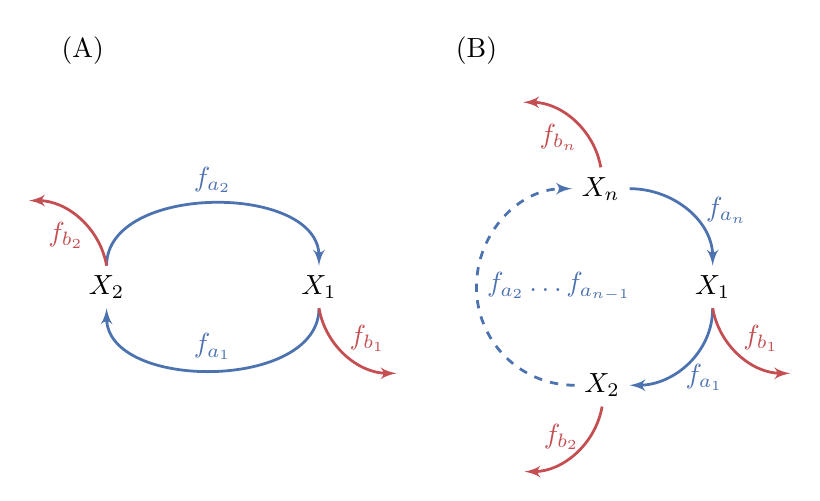
\begin{tikzpicture}[>=latex']
    \begin{scope}[shift={(-5cm,0cm)},node distance = 2cm]
        \node (X1) {$X_1$};
        \node[left=of X1]  (X2) {$X_2$};
        \draw [->,line width=1pt,autocatacyc] (X1.south) [out=-90,in=-90] to  node [pos=0.5,above] (fa1) {$f_{a_1}$} (X2.south);
        \draw [->,line width=1pt,autocatacyc] (X2.north) [out=90,in=90] to  node [pos=0.5,above] (fa2) {$f_{a_2}$} (X1.north);
        \draw [->,line width=1pt,branchout] (X1.south) arc (190:270:1cm) node [pos=0.3,right,xshift=1mm] {$f_{b_1}$};
        \draw [->,line width=1pt,branchout] (X2.north) arc (10:90:1cm) node [pos=0.3,left] {$f_{b_2}$};
    \end{scope}
    \begin{scope}[shift={(0cm,0cm)},node distance = 1cm]
        \node (X1) {$X_1$};
        \node[below left=of X1]  (X2) {$X_2$};
        \node[above left=of X1]  (Xn) {$X_n$};
        \draw [->,line width=1pt,autocatacyc] (X1.south) [out=-90,in=0] to  node [pos=0.7,right,xshift=1mm] (fa1) {$f_{a_1}$} (X2.east);
        \draw [->,line width=1pt,autocatacyc] (Xn.east) [out=0,in=90] to  node [pos=0.5,right,xshift=1mm] (fan) {$f_{a_n}$} (X1.north);
        \draw [->,line width=1pt,branchout] (X1.south) arc (190:270:1cm) node [pos=0.3,right,xshift=1mm] {$f_{b_1}$};
        \draw [->,line width=1pt,branchout] (X2.south) arc (-10:-90:1cm) node [pos=0.3,left] {$f_{b_2}$};
        \draw [->,line width=1pt,branchout] (Xn.north) arc (10:90:1cm) node [pos=0.3,left] {$f_{b_n}$};
        \draw [->,line width=1pt,autocatacyc,dashed] (X2.west) [out=180,in=-90] to ($(X1)+(-3,0)$) node [right] (fmid) {$f_{a_2}\dots f_{a_{n-1}}$} to [out=90,in=180] (Xn.west);
    \end{scope}
    \iftoggle{article} {
        \node [shift={(-8cm,3cm)}] (A) {(A)};
        \node [right of=A,xshift=4cm] (B) {(B)};
    }{}
\end{tikzpicture}


     \caption{Multiple-reaction autocatalytic cycles. (A) A two reaction system. (B) A generic $n$-reaction system. A sufficient condition for the stability of a steady state point in such systems is that the elasticity of each biomass generating reaction is larger than or equal to the elasticity of the equivalent autocatalytic reaction at the steady state concentration.}
     \label{fig:multiple}
\end{figure}
    \subsubsection{Using different kinetics equations}
    Although we utilized the widely-used irreversible Michaelis-Menten kinetics equation to model enzyme kinetics, our results can be extended to different kinetic equations.
    Generally, two conditions must be met for a stable flux through an autocatalytic cycle to exist: (A) there should be a positive concentration of the intermediate metabolites for which the outgoing fluxes balance the autocatalytic fluxes, resulting in a steady state of fluxes, and, (B) at the steady state point the combined elasticities of all the outgoing reactions out of the cycle should be higher than the elasticities of the autocatalytic reactions, as is implied by equation \ref{eq:complex}, to enforce stability in the presence of small perturbations.
    Therefore, these two conditions should be explicitly evaluated for every case with different kinetic equations and autocatalytic cycles topologies to assert whether it can carry stable fluxes or not.

    Two guideline observations can be extracted, regardless of the exact kinetic behavior of the relevant enzymes:
    \begin{enumerate}
        \item If a positive flux steady state exists, and the branching reactions have higher $V_{\max}$ values than the autocatalytic reactions, then a positive stable flux steady state is attainable (though it may not necessarily be the same steady state).
        This claim can be deduced as follows:
        If the given steady state is stable, then the claim is obviously correct.
        Otherwise, the given steady state is unstable, so for concentrations slightly above the steady state concentrations, the autocatalytic reactions will drive the intermediate metabolites concentrations to even higher values.
        However, for large enough concentrations of intermediate metabolites the branching reactions will carry higher flux than the autocatalytic reactions, as their $V_{\max}$ values are higher, driving the concentrations of intermediate metabolites down.
        There must therefore be some threshold concentration value below which the autocatalytic reactions carry higher flux, and above which the branching reactions carry higher flux, making this threshold concentration point a stable steady state.
    \item For concentration domains at which the kinetic function of an enzyme is concave, the elasticity of the reaction is anti correlated with the level of saturation of the reaction (where the level of saturation of a reaction is defined as the ratio between the flux through the reaction and the maximal flux it can carry, $V_{\max}$), meaning that the more saturated the reaction is, the lower is its elasticity and vice versa.
          This mathematical property of concave, monotonically increasing, bounded functions clearly follows from the observation that the first derivative of a concave function is a decreasing function, whereas the value of the function, by definition, is an increasing function. 
          As the function is bounded, its saturation is also an increasing function, resulting in an anti correlation between the saturation level and the derivative.
    \end{enumerate}

    These guidelines give a basis for evaluating the stability of operational autocatalytic cycles given fluxomics and proteomics data as is demonstrated below.

    While these guidelines offer sufficient conditions for stability, they are not necessary, meaning a stable steady state can be achieved even in cases where these conditions are not met, or, for example, in cases where the kinetic equations follow a hill function with a coefficient that is larger than 1, making them convex for at least some domain of positive substrate concentrations.
    However, we can conclude from this analysis that the branching reactions out of a cycle, having a large elasticity at the steady state concentration, cannot be saturated at that point, meaning the enzymes driving the flux out of the cycle and through these reactions are under-utilized resulting in an inherent seeming inefficiency.
    In physiological context this effect is expected to be even higher as the expression pattern of the enzymes must ensure stable fluxes even under expression noise that may alter the amount of both the autocatalytic and the branching reactions enzymes, requiring a large 'buffer zone' to be maintained between the maximal capacity of the branching reactions enzymes versus that of the autocatalytic reactions enzymes.

    \subsection{Testing the predictions of the analysis with experimental data on functioning autocatalytic cycles}
    To evaluate the validity of our analysis of autocatalytic cycles we searched for growth conditions under which the autocatalytic cycles we identified in central carbon metabolism carry substantial flux in vivo.
    We used recent in-vivo flux measurements from \cite{Gerosa2015-oq}.  
    According to the measurements, two classes of autocatalytic cycles carry substantial flux under at least one of the growth conditions used in \cite{Gerosa2015-oq}:
    cycles using the PTS transport system carry significant flux at growth in glucose and fructose;
    the glyoxylate cycle carries significant flux at growth in galactose and acetate.

    The PP cycle variants do not carry flux in any of the measured conditions, which is expected given the non-standard metabolites most of their variants assimilate.
    The only physiologically reasonable configuration under which a PP autocatalytic cycle would carry flux is in growth under ribose while missing the rpi reaction, a condition for which no fluxomics measurements are currently available.

    The reverse FBA with ED pathway cycle did not carry flux in any of the measured conditions.
    Although glycerol could have been a potential carbon source to use this pathway, the metabolic network allows for a more energy efficient growth by using the tpi reaction, following the common lower glycolysis reactions from GAP to pyruvate, avoiding the need to use the less energy efficient ED pathway.

    As noted above, two guidelines for evaluating stability can be explored at major branch points out of a functioning autocatalytic cycle: (A) the maximal flux of the branching reaction, $V_{\max,b}$ should be higher than the maximal flux of the corresponding autocatalytic reaction, $V_{\max,a}$, and, (B) the saturation of the branching reaction should be higher than the saturation of the corresponding autocatalytic reaction.
    We stress again that these conditions are sufficient, but not necessary, for the autocatalytic cycle to be at a stable steady state point.

    To estimate the maximal capacity of a reaction, $V_{\max}$ we followed the procedure described in \cite{Davidi2016-ga}.
    Briefly, for each reaction, under every condition we divided the flux the reaction carries (obtained from \cite{Gerosa2015-oq}) by the amount of the corresponding enzyme expressed under that condition.
    We used data from \cite{Schmidt2015} to obtain the enzyme expression level.
    We thus got a flux per enzyme estimate for the given reaction under each of the conditions.
    We defined the enzyme maximal capacity as the maximum flux per unit enzyme it carries across all reactions.
    Multiplying the enzyme maximal capacity by the enzyme amount at each condition therefore results in an estimate of the maximal possible flux through the given reaction under the relevant condition.


    We used the data from \cite{Gerosa2015-oq} to identify the major branch points in each functioning cycle and the flux distributions in them under each of the relevant conditions.
    The results are presented in figure \ref{fig:branch}.
    The results show that for every functioning autocatalytic cycle, in at least one branch point the biomass generating reaction has a larger maximal flux capacity, and is considerably less saturated than the respective autocatalytic reaction.
    Moreover, out of 9 branch points analyzed, in 6 branch points the branching reactions were significantly less saturated than the autocatalytic reactions, in 2 branch points the saturation levels were similar, and only in one branch point the auto catalytic reaction was less saturated than the branching reaction.
    The branch point that does not agree with our prediction is the branch point in fructose-1,6-bisphosphate at growth with fructose as the carbon source.
    The disagreement arises as a large flux is assigned to the fbp reaction, whereas the corresponding enzyme is not highly expressed.
    This disagreement may be the result of neglecting transport of fructose as fructose-6-phosphate, and not fructose-1,6-bisphosphate, which is known to occur in the concentration at which the measurements were made \cite{Kornberg1990-ft}, and which was neglected in \cite{Gerosa2015-oq}.
    Assuming $20\%$ of transported fructose is converted directly to f6p suffices in order to resolve the disagreement, resulting in equal saturation levels for the autocatalytic reaction and the branching reaction.

    The lower saturation values of biomass generating reactions demonstrate that the expressed enzymes have enough capacity to prevent the autocatalytic cycle from increasing the concentration of intermediate metabolites infinitely.
    Moreover, the lower saturation values of the biomass generating reactions suggest that at the steady state point their elasticities are higher, ensuring stable operation of the cycle.

    Another demonstration of the autocatalytic mechanism being at play is in the CBB cycle, which is not a part of the metabolic network of wild type \emph{E.coli}, and for which no flux measurements are available.
    This cycle has been recently introduced synthetically into \emph{E.coli} and was shown to carry flux in it, given further metabolic engineering of central carbon metabolism \cite{Antonovski2016}.
    The experimentally observed key evolutionary event enabling the functioning of the CBB cycle, was a mutation affecting the kinetic properties of the main branching reaction out of the CBB pathway, PRS, reducing its affinity to its substrate, ribose-5p.

    To conclude, while thorough knowledge of the kinetic properties, concentrations and fluxes under various growth conditions is sparse, existing data supports predictions made by our model, given the requirement for stable steady state operation of autocatalytic cycles.
    The model can therefore be used to shed more light on seemingly wasteful investment in the expression of enzymes the capacity of which is not fully utilized, as well as for highlighting at what metabolic branch points enzymes kinetic efficiency may be constrained due to stability requirements of a corresponding autocatalytic cycle.

\begin{figure}[h!]
\centering
\resizebox{1\linewidth}{!}{
    \input{experimental-fluxes.tex}
}
\caption{
  Major branch points and relative enzyme saturation in operating autocatalytic cycles.
  In all cases there is enough excess capacity in the branching reactions to prevent the cycle from overflowing.
  A $4\%$ flux from pep to biomass was neglected in growth under glucose and fructose.
  Only in one out of the 8 branch points observed (the branch point at fbp in growth under fructose), the outgoing reaction is significantly more saturated than the autocatalytic reaction.
  (*) A branch point at which the branching reaction is more saturated than the autocatalytic reaction, which may result from neglecting fructose transport directly as f6p when deriving fluxes (see text).
}
    \label{fig:branch}
\end{figure}


\section{Discussion}
Our study into the dynamics and stability of autocatalytic cycles suggests design principles applicable to both synthetic biology in the effort to express novel heterologous cycles and in the context of systems biology that aims to understand the function of natural networks.
A common concept in synthetic biology is that the successful implementation of novel pathways requires the expression of functional enzymes in the correct amounts in the target organism.
Here we show that in the context of autocatalytic cycles, such a successful expression may not suffice.
Specifically, changes to some of the kinetic parameters of enzymes at branch points of the cycle may be required in order for the novel pathway to function.

Another aspect of our findings is that while it is common to assume that high affinity and catalytic rate are desirable traits for enzymes, in the context of autocatalytic cycles, constraints may exist on the relations between these kinetic parameters across different enzymes rendering improvements in some of them deleterious for the functioning of the cycle.
Moreover, in order for a cycle to be stable, at least some of the enzymes catalyzing reactions out of the cycles may need to be over-expressed, resulting in a seemingly inefficient expression pattern that is required in order to ensure that branching reactions are less saturated than the corresponding autocatalytic reactions.

A recent demonstration of these principles in vivo is the implementation of a functional CBB cycle in \emph{E.coli} by introducing the two genes missing for its function \cite{Antonovski2016}.
The successful introduction of the genes did not suffice to make the cycle function, and further directed evolution was needed in order to achieve successful operation of the cycle.
Most changes occurred in branch points from the cycle.
The change which was biochemically characterized in the evolutionary process was the decrease of the affinity of phosphoribosylpyrophosphate synthetase (PRS), one of the enzymes responsible for flux out of the CBB cycle, corresponding to the biomass reaction in our simple model.
This is beautifully in line with the predictions of our analysis that suggests that a decrease in the $\sfrac{K_{\text{cat}}}{K_M}$ of the branching reaction out reaction is the change that will lead to existence and stability of a solution.

Our observation regarding the stabilizing effect of input fluxes into an autocatalytic cycle may provide some means to mitigate the stability issue in synthetic biology metabolic engineering setups, allowing for a pathway to gradually evolve towards sustainable, substantial flux.

While autocatalytic cycles are usually considered a small part of metabolism, we find that such cycles are at the heart of central carbon metabolism.
The examples of autocatalytic cycles we provide, as well as our verified predictions on the usage of enzymes catalyzing reactions branching out of such cycles, suggest that the constraints we find on the kinetic parameters of enzymes involved in autocatalytic cycles may shape the kinetic parameters of a broad set of enzymes central to metabolism.

  Finally, while our work focuses on cycles increasing the amount of carbon in the system, we note that autocatalysis can be defined with respect to other quantities such as energy (e.g. ATP investment and the production in glycolysis), non-carbon atoms, reducing power, or other moieties \cite{Reich1981-qd}.
  The analysis we present here can thus be of even wider relevance for the design and analysis of metabolic networks.

  \section{Methods}
  \subsection{Systematic identification of autocatalytic cycles in metabolic networks}
  We implemeneted an algorithm to systematically search for autocatalytic cycles in metabolic networks.
  The algorithm is incomplete, meaning there may be autocatalytic cycles that will not be identified by it.
  In our framework, a metabolic network is defined by a set of reactions, $(R)$.
  Each reaction is defined by a set of substrates and a set of products, with corresponding stoichiometries $R_i=(S,P,N^S,N^P)$, such that $R_i$ describes the reaction $\sum_j N_j^SS_j \rightarrow \sum_k N_k^PP_k$.
  The algorithm works as follows:
  \begin{enumerate}
    \item All co-factors are removed from the description of the metabolic network, so that it is carbon-based.
    \item The metabolic network is converted to a directed graph, G:
  The nodes of G are all the metabolites and all the reactions of the network.
  For each metabolite, $M$, and each reaction, $R$, if $M$ is a substrate of $R$ then the edge $(M,R)$ is added to the graph, and if $M$ is a product of $R$, then the edge $(R,M)$ is added to the graph.
    \item The Tarajan cycle identification algorithm is used to enumerate all the cycles in the graph.
    \item for every cycle identified by the Tarajan algorithm, $C$, the algorithm checks if the cycle can be the backbone of an auto catalytic cycle as follows:
        \begin{enumerate}
            \item For every reaction in the cycle, $R$, the algorithm checks if it consumes more than one  intermediate metabolite of the cycle.
              If so, $C$ is assumed not to be autocatalytic and the algorithm continues to evaluate the next cycle.
            \item Otherwise, for every reaction in the cycle, $R$, the algorithm checks if it has more than one product that is an intermediate metabolite of the cycle.
              If so, then the algorithm lists $C$ as an autocatalytic cycle.
            \item Finally, the algorithm checks, for every reaction in the cycle, if it has a product that is not an intermediate metabolites of the cycle.
                If so, denote by $M_E$ such a metabolite.
            The algorithm proceeds to check if, for every intermediate metabolite of the cycle, $M_i$ a reaction exists from $M_E$ to $M_i$ that does not use any of the reactions of the cycle, and does not consume any of the intermediate metabolites of the cycle.
            If so then the algorithm lists $C$ as an autocatalytic cycle.
        \end{enumerate}
  \end{enumerate}

  The algorithm assumes reactions consume exactly one molecule of any of their substrates and produces exactly one molecule of any of their products, an assumption that is valid in central carbon metabolism, but not in metabolic networks in general.
  
    \subsection{For Michaelis-Menten kinetics, relation of derivatives result in inverse relation of saturation levels}
    It turnes out that for the Michaelis-Menten kinetics equations, the following useful lemma can be used to connect theoretical observations on the relations of derivatives to physiological observations on saturation levels.

    We define the saturation level of a reaction as the ratio between the flux it carries, and the maximal flux it can carry, given the expression level of the relevant enzyme, that is:
    \begin{equation*}
      S(X)=\frac{f(X)}{V_{\max}}=\frac{X}{K_M+X}
    \end{equation*}

    Given this definition we can show that if two Michaelis-Menten reactions consume the same metabolite, $X$, and at a given concentration, $X^*$, it holds that $f_a(X^*)\geq f_b(X^*)$, then if:
    \begin{equation}
        \frac{df_b}{dX}\Big\vert_{X^*}>\frac{df_a}{dX}\Big\vert_{X^*}
        \label{eq:lemmapremise}
    \end{equation}
    then it follows that:
    \begin{equation*}
        S_b(X^*)<S_a(X^*)
    \end{equation*}
    Proof: expanding the condition that $f_a(X^*)\geq f_b(X^*)$, we get that:
    \begin{equation}
        \frac{V_{\max,b}X^*}{K_{M,b}+X^*}\leq\frac{V_{\max,a}X^*}{K_{M,a}+X^*} \rightarrow
         \frac{V_{\max,b}}{K_{M,b}+X^*}\leq\frac{V_{\max,a}}{K_{M,a}+X^*}
         \label{eq:firstmid}
     \end{equation}
     Expanding the premise of the lemma in equation \ref{eq:lemmapremise} gives us that:
     \begin{equation*}
        \frac{df_b}{dX}\Big\vert_{X^*}>\frac{df_a}{dX}\Big\vert_{X^*} \rightarrow
        \frac{V_{\max,b}K_{M,b}}{(K_{M,b}+X^*)^2} > \frac{V_{\max,a}K_{M,a}}{(K_{M,a}+X^*)^2}
     \end{equation*}
     Because equation \ref{eq:firstmid} holds, it follows that:
     \begin{equation*}
         \frac{K_{M,b}}{K_{M,b}+X^*} > \frac{K_{M,a}}{K_{M,a}+X^*} \rightarrow \frac{1}{1+\frac{X^*}{K_{M,b}}} > \frac{1}{1+\frac{X^*}{K_{M,a}}} \rightarrow K_{M,b}>K_{M,a}
     \end{equation*}
    Finally, we note that:
    \begin{equation*}
        K_{M,b}>K_{M,a} \rightarrow X^*+K_{M,b}>X^*+K_{M,a} \rightarrow \frac{X^*}{X^*+K_{M,b}}<\frac{X^*}{X^*+K_{M,a} } \rightarrow S_b(X^*)<S_a(X^*)
    \end{equation*}
    concluding the proof.

     If we now assume that a complex system is at a stable steady state point, such that it satisfies equations \ref{eq:complexstst} and \ref{eq:complexstab}, we get that:
    \begin{equation*}
      \beta \geq \alpha \rightarrow
      \frac{V_{\max,b}K_{M,b}}{(K_{M,b}+X)^2} \geq \frac{V_{\max,a}K_{M,a}}{(K_{M,a}+X)^2}
    \end{equation*}
    \begin{equation*}
     f_b\leq f_a \rightarrow
     \frac{V_{\max,b}X}{K_{M,b}+X}\leq\frac{V_{\max,a}X}{K_{M,a}+X} \rightarrow
     \frac{V_{\max,b}}{K_{M,b}+X}\leq\frac{V_{\max,a}}{K_{M,a}+X}
    \end{equation*}
    Combining these two equations we get that:
    \begin{equation*}
    \begin{dcases}
      & \frac{V_{\max,b}}{K_{M,b}+X}\leq\frac{V_{\max,a}}{K_{M,a}+X} \\
      & \frac{V_{\max,b}K_{M,b}}{(K_{M,b}+X)^2} \geq \frac{V_{\max,a}K_{M,a}}{(K_{M,a}+X)^2}
    \end{dcases}
    \end{equation*}
    Substituting the first equation into the second one we deduce that:
    \begin{equation*}
      \frac{K_{M,b}}{K_{M,b}+X} \geq \frac{K_{M,a}}{K_{M,a}+X}\rightarrow K_{M,b}\geq K_{M,a}
    \end{equation*}
    Now we can finish the derivation as:
    \begin{equation*}
      K_{M,b}\geq K_{M,a} \rightarrow  K_{M,b}+X\geq K_{M,a}+X \rightarrow \frac{1}{ K_{M,a}+X} \geq \frac{1}{ K_{M,b}+X} \rightarrow \frac{X}{ K_{M,a}+X} \geq \frac{X}{ K_{M,b}+X} \rightarrow S_a \geq S_b
    \end{equation*}

\newpage
\section{Appendices}
\begin{figure}[H]
    \iftoggle{elifesubmission} { }
    {
    \centering{
        \input{extra-cycles-figure1.tex}}
    }
\caption{
    \label{fig:extrasamps1}
    An autocatalytic cycle assimilating ribose-5-phosphate using the pentose phosphate pathway.
    This cycle contains a direct input reaction (rpi, dashed line) allowing the cycle to operate with broader sets of kinetic parameters than cycles missing this feature.
    A knockout strain where rpi is eliminated, does not grow under ribose despite having the theoretical ability to do so.
}
\end{figure}
\begin{figure}[H]
    \iftoggle{elifesubmission} { }
    {
    \centering{
        \input{extra-cycles-figure2.tex}}
    }
\caption{
    \label{fig:extrasamps2}
    An autocatalytic cycle assimilating dhap while consuming gap using the fba reaction in the gluconeogenic direction.
    This cycle contains a direct input reaction (tpi, dashed line) allowing the cycle to operate with broader sets of kinetic parameters than cycles missing this feature.
    Accurding to fluxomics data this cycle does not operate in vivo as a more energy efficient alternative in growth under glycerol is to use the tpi reaction and proceed in the glycolitic direction in the lower part of glycolysis.
    A knockout strain where tpi reaction is eliminated, does not grow under glycerol despite having the theoretical ability to do so.
}
\end{figure}
\iftoggle{elifesubmission} {
    \subsubsection{Supplementary File 1}
    Supplementary File 1 contains the tables used in the data analysis in this work.
    The ``contents'' sheet includes the description of the different tables and is provided here as well:
    \begin{itemize}
        \item Fluxes source: The metabolic fluxes sheet from Data S1 in \cite{Gerosa2015-oq}.
        \item Cell size source: The cell sizes used for calculations as taken from Supplementary tables, Table ``Content and abbrevations'' in \cite{Schmidt2015}.
        \item Protein abundance: Protein abundance data from Supplementary tables, Table S6 in \cite{Schmidt2015}.
        \item Reaction-Protein mapping: Mapping between reactions and genes of catalyzing enzymes.
        \item Flux per enzyme: Calculation of the flux per enzyme for all the reactions listed in the ``Reaction-Protein mapping'' table.
        \item Reaction Saturation: Estimated saturation of enzymes across conditions.
        \item Non autocatalytic cycles reaction saturation: Comparison of saturation levels of branch versus cycle reactions for non-autocatalytic cycles.
        \item Allosteric regulation: Listing allosteric interactions between autocatalytic components.
    \end{itemize}
}
{
%    \begin{figure}[H]
%    \centering{
%\input{atp-cycle.tex}
%}
%\caption{
% ATP autocatalysis in glycolysis.
% This autocatalytic cycle considers high energy phosphate bonds as the moiety that is required for the production of larger quantities of high energy phosphate bonds.
% Cycle intermediates are black, external metabolites are gray.
% The high energy bonds of ADP are neglected.
% The total autocatalytic reaction is: $2\text{ATP}+\text{gluc}+2\text{P}_i+2\text{ADP}\rightarrow 4\text{ATP}+2\text{pyr}$ (neglecting the double nad $\rightarrow$ nadh reaction coupled to the gap $\rightarrow$ bpg reaction).
% }
%\end{figure}
%\subsection{Analysis of a simple cycle with reversible branch reaction}
We analyze the simple autocatalytic cycle, with a reversible branch reaction, presented in figure \ref{fig:reversible}.
\begin{figure}[!htb]
  \centering
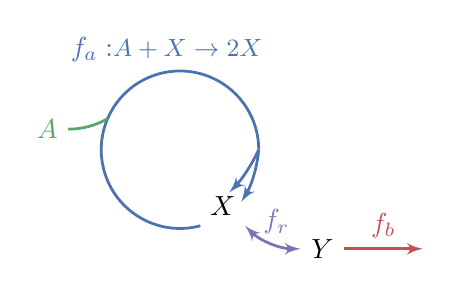
\begin{tikzpicture}[>=latex']
    \begin{scope}%[node distance = 2cm]
        \node at (-60:1cm) (X) {$X$};
        \node[shape=coordinate] (orig) {};
        \draw [-,line width=1pt,autocatacyc] (X.south west) arc (285:0:1cm) node [pos=0.65,above] (fa) {$f_a:$\small{$A+X\rightarrow2X$}} node [pos=0.45,shape=coordinate] (midauto) {} node [pos=1,shape=coordinate] (endcommon) {};
        \draw [->,line width=1pt,autocatacyc] (endcommon) arc (-25:-44:2cm);
        \draw [->,line width=1pt,autocatacyc] (endcommon) arc (-5:-32:1.5cm);
        \draw [line width=1pt,assimcol] (midauto) arc (-60:-90:1cm) node [pos=1,left] (e) {$A$};
        \draw [<->,line width=1pt,magenta] (X.south east) arc (225:270:1cm) node [pos=0.6,above] {$f_r$} node [pos=1,right,black] (Y) {$Y$};
        \node[right=of Y, shape=coordinate] (out) {};
        \draw [->,line width=1pt,branchout] (Y) -- node [pos=0.5,above] {$f_b$}(out);
    \end{scope}
\end{tikzpicture}
     \caption{
         A simple autocatalytic cycle with a reversible branch reaction
     \label{fig:reversible}
 }

\end{figure}

\subsubsection{Steady state existance conditions}
We assume that $K_{\text{eq}}=1$.
As at a positive steady state, $f_r>0$, it follows that $X>Y$.
Because at steady state it also holds that $f_a$=$f_b$, it follows that $f_b$ attains the same flux as $f_a$ under a lower concentration of its substrate.
It must therefore hold that either $V_{\max,a}/K_{M,a}<V_{\max,b}/K_{M,b}$, or $V_{\max,a}<V_{\max,b}$ (or both).
Visually, this implies that case (IV) in figure \ref{fig:simplecycle} is eliminated.

The reversible Michaelis Menten equation (assuming $K_{\text{eq}}=1$)  states that:

\begin{equation*}
  f(X,Y)=\frac{\frac{V_{\max}}{K_{M,X}}(X-Y)}{1+\frac{X}{K_{M,X}}+\frac{Y}{K_{M,Y}}} = \frac{V_{\max}(X-Y)}{K_{M,X}+X+\frac{K_{M,X}Y}{K_{M,Y}}} 
\end{equation*}

In this case, if the branch reaction is reversible, then for every concentration of the intermediate metabolite $X$, $Y$ must allow the reversible flux to balance the autocatalytic flux:
\begin{equation*}
  f_a(X)=f(X,Y)\Rightarrow \frac{V_{\max,a}X}{K_{M,a}+X}=\frac{V_{\max}(X-Y)}{K_{M,X}+X+\frac{K_{M,X}Y}{K_{M,Y}}}
\end{equation*}

which implies:

\begin{equation*}
  -\frac{V_{\max,a}X}{K_{M,a}+X}(K_{M,X}+X)+V_{\max}X=V_{\max}Y+\frac{V_{\max,a}X}{K_{M,a}+X}\frac{K_{M,X}Y}{K_{M,Y}}
\end{equation*}
That results in:
\begin{equation*}
  \frac{V_{\max}X-\frac{V_{\max,a}X}{K_{M,a}+X}(K_{M,X}+X)}{V_{\max}+\frac{K_{M,X}V_{\max,a}X}{K_{M,Y}(K_{M,a}+X)}}=Y
\end{equation*}

That is equal to:
\begin{equation*}
  \frac{V_{\max}X(K_{M,a}+X)-V_{\max,a}X(K_{M,X}+X)}{V_{\max}(K_{M,a}+X)+\frac{K_{M,X}V_{\max,a}X}{K_{M,Y}}}=Y
\end{equation*}
As $Y>0$ at the steady state, it follows that:
\begin{equation*}
  V_{\max}(K_{M,a}+X)-V_{\max,a}(K_{M,X}+X)>0 \Rightarrow \frac{V_{\max}}{K_{M,X}+X}>\frac{V_{\max,a}}{K_{M,a}+X}
\end{equation*}
which implies that at least one of the two inequations must hold for a solution to exist:
\begin{align*}
  V_{\max} &> V_{\max,a} \\
  \frac{V_{\max}}{K_{M,X}} &>\frac{V_{\max,a}}{K_{M,a}}
\end{align*}


For a concentration to represent a steady state it must also hold that $f_b(Y)=f_a(X)$, so:
\begin{equation*}
    \frac{V_{\max,a}X}{K_{M,a}+X}=\frac{V_{\max,b}Y}{K_{M,b}+Y}
\end{equation*}
which results in:
\begin{equation*}
    K_{M,b}\frac{V_{\max,a}X}{K_{M,a}+X}=Y(V_{\max,b}-\frac{V_{\max,a}X}{K_{M,a}+X})
\end{equation*}
That can be simplified to:
\begin{equation*}
    \frac{K_{M,b}V_{\max,a}X}{V_{\max,b}(K_{M,a}+X)-V_{\max,a}X}=Y
\end{equation*}
As here, again, $Y>0$, it follows that:
\begin{equation*}
  V_{\max,b}>\frac{V_{\max,a}X}{K_{M,a}+X}
\end{equation*}


Combining the two conditions yields that at steady state $X$ satisfies:
\begin{equation*}
    \frac{K_{M,b}V_{\max,a}X}{V_{\max,b}(K_{M,a}+X)-V_{\max,a}X}=\frac{XV_{\max}(K_{M,a}+X)-XV_{\max,a}(K_{M,X}+X)}{V_{\max}(K_{M,a}+X)+\frac{K_{M,X}V_{\max,a}X}{K_{M,Y}}}
\end{equation*}

So $X=0$ is a steady state and for the other solution we get:
\begin{equation*}
    \frac{K_{M,b}V_{\max,a}}{V_{\max,b}K_{M,a}+(V_{\max,b}-V_{\max,a})X}=\frac{V_{\max}K_{M,a}-V_{\max,a}K_{M,X}+(V_{\max}-V_{\max,a})X}{V_{\max}K_{M,a}+(V_{\max}+\frac{K_{M,X}V_{\max,a}}{K_{M,Y}})X}
\end{equation*}

Where the solutions to this equation must yield $X>0$ and $Y>0$.

%Simplifying give:
%\begin{equation*}
%  K_{M,b}V_{\max,a}
%  V_{\max}K_{M,a}+
%  K_{M,b}V_{\max,a}
%  (V_{\max}+\frac{K_{M,X}V_{\max,a}}{K_{M,Y}})X=
%  (V_{\max,b}K_{M,a}+(V_{\max,b}-V_{\max,a})X)
%  (V_{\max}K_{M,a}-V_{\max,a}K_{M,X}+(V_{\max}-V_{\max,a})X)
%\end{equation*}

\subsubsection{Stability analysis of a steady state}
For a steady state to be stable, the eigenvalues of the Jacobian matrix must have negative real values.
In our system it holds that:
    \begin{align*}
        \dot{X} & =f_a-f_r \\
        \dot{Y} & =f_r-f_b
    \end{align*}
We use the following notation:
\begin{align*}
  \alpha & =\frac{df_a}{dX}=\frac{V_{\max,a}K_{M,a}}{(K_{M,a}+X)^2} \\
  \beta & =\frac{df_b}{dY}=\frac{V_{\max,b}K_{M,b}}{(K_{M,b}+X)^2} \\
  \gamma_x & =\frac{\partial f_r}{\partial X}= \frac{V_{\max}(K_{M,X}+Y(1+\frac{K_{M,X}}{K_{M,Y}}))}{(K_{M,X}+X+\frac{K_{M,X}Y}{K_{M,Y}})^2}
\\
  \gamma_y & =\frac{\partial f_r}{\partial Y}= \frac{-V_{\max}(K_{M,X}+X(1+\frac{K_{M,X}}{K_{M,Y}}))}{(K_{M,X}+X+\frac{K_{M,X}Y}{K_{M,Y}})^2} 
\end{align*}

We note that for MM kinetics and positive concentrations it holds that:
    \begin{align*}
        \alpha & >0 \\
        \beta & >0 \\
        \gamma_x & >0 \\
        -\gamma_y & >\gamma_x \\
    \end{align*}

We can use this notation to write the Jacobian matrix as:
   \begin{equation*}
        J=
        \begin{pmatrix}
            \alpha-\gamma_x & -\gamma_y \\
            \gamma_x & \gamma_y-\beta
        \end{pmatrix}
    \end{equation*}
which gives a characteristic polynomial of:
\begin{equation*}
    (\alpha-\gamma_x-\lambda)(\gamma_y-\beta-\lambda)+\gamma_y\gamma_x=0
\end{equation*}
In order for the real values of the roots of the characteristic polynomial to be negative it must hold that $b>0$ and $c>0$, where $b$ and $c$ are the coefficients of the quadratic equation $a\lambda^2+b\lambda+c=0$.
We therefore get that:
\begin{align*}
b & =\gamma_x-\alpha-\gamma_y+\beta>0\\
c & =(\alpha-\gamma_x)(\gamma_y-\beta)+\gamma_y\gamma_x>0
\end{align*}
We note that as $\gamma_y\gamma_x<0$ and $\gamma_y-\beta<0$, it is a necessary, but not sufficient, condition that $\alpha-\gamma_x<0$ for the second inequality to hold.
This is also a sufficient condition for the first inequality to hold.
The sufficient condition for the second inequality to hold is that:
\begin{equation*}
  \gamma_x-\alpha>\gamma_y\gamma_x/(\gamma_y-\beta)=\frac{\gamma_x}{1-\frac{\beta}{\gamma_y}}\Rightarrow (1-\frac{\alpha}{\gamma_x})(1-\frac{\beta}{\gamma_y})>1
\end{equation*}
which implies that the smaller $\beta$ is, the larger the ratio between $\gamma_x$ and $\alpha$ needs to be in order to ensure stability.
Moreover, as $-\gamma_y >\gamma_x$ it follows that $\beta>\alpha$.
We can use the last inequality to get that:
\begin{equation*}
    \beta>\alpha \Rightarrow \frac{V_{\max,b}K_{M,b}}{(K_{M,b}+X)^2}>\frac{V_{\max,a}K_{M,a}}{(K_{M,a}+X)^2} \Rightarrow \frac{V_{\max,b}XK_{M,b}}{(K_{M,b}+X)^2}>\frac{V_{\max,a}XK_{M,a}}{(K_{M,a}+X)^2} \Rightarrow f_b(X)\frac{K_{M,b}}{K_{M,b}+X}>f_a(X)\frac{K_{M,a}}{K_{M,a}+X}
\end{equation*}
But, since $f_a(X)=f_b(X)$ at the steady state point we can simplify and get:
\begin{equation*}
    \frac{K_{M,b}}{K_{M,b}+X}>\frac{K_{M,a}}{K_{M,a}+X} \Rightarrow \frac{1}{1+X/K_{M,b}}>\frac{1}{1+X/K_{M,a}} \Rightarrow K_{M,b}>K_{M,a}
\end{equation*}
From the fact that $\alpha<\gamma_x$ we can similarly get that:
\begin{align*}
\alpha<\gamma_x \Rightarrow
\frac{V_{\max,a}K_{M,a}}{(K_{M,a}+X)^2} < \frac{V_{\max}(K_{M,X}+Y(1+\frac{K_{M,X}}{K_{M,Y}}))}{(K_{M,X}+X+\frac{K_{M,X}Y}{K_{M,Y}})^2}
\Rightarrow \\
\frac{V_{\max,a}XK_{M,a}}{(K_{M,a}+X)^2}<\frac{V_{\max}X(K_{M,X}+Y(1+\frac{K_{M,X}}{K_{M,Y}}))}{(K_{M,X}+X+\frac{K_{M,X}Y}{K_{M,Y}})^2}
\Rightarrow \\
f_r(X)\frac{K_{M,a}}{K_{M,a}+X}<\frac{V_{\max}X(K_{M,X}+Y(1+\frac{K_{M,X}}{K_{M,Y}}))}{(K_{M,X}+X+\frac{K_{M,X}Y}{K_{M,Y}})^2}
\end{align*}
So we get:
\begin{equation*}
\frac{V_{\max}(X-Y)}{K_{M,X}+X+\frac{K_{M,X}Y}{K_{M,Y}}}\frac{K_{M,a}}{K_{M,a}+X}<\frac{V_{\max}X(K_{M,X}+Y(1+\frac{K_{M,X}}{K_{M,Y}}))}{(K_{M,X}+X+\frac{K_{M,X}Y}{K_{M,Y}})^2}
\end{equation*}
that can be simplified to:
\begin{equation*}
\frac{(X-Y)}{1}\frac{K_{M,a}}{K_{M,a}+X}<\frac{X(K_{M,X}+Y(1+\frac{K_{M,X}}{K_{M,Y}}))}{K_{M,X}+X+\frac{K_{M,X}Y}{K_{M,Y}}}
\end{equation*}
And further to:
\begin{equation*}
    \frac{(X-Y)}{1}\frac{K_{M,a}}{V_{\max,a}X}<\frac{X(K_{M,X}+Y(1+\frac{K_{M,X}}{K_{M,Y}}))}{V_{\max}(X-Y)}
\end{equation*}
\subsubsection{Conclusion}
In this case for a positive steady state to exist it must hold that:
\begin{align*}
    &\begin{dcases}
        V_{\max,b} &> V_{\max,a} \quad \text{or}, \\
        \frac{V_{\max,b}}{K_{M,b}} &>\frac{V_{\max,a}}{K_{M,a}}
    \end{dcases}\\
    &\text{and} \\
  &\begin{dcases}
        V_{\max} &> V_{\max,a} \quad \text{or}, \\
        \frac{V_{\max}}{K_{M,X}} &>\frac{V_{\max,a}}{K_{M,a}}
    \end{dcases}
\end{align*}

For the positive steady state to be stable, it must hold that:
\begin{align*}
(1-\frac{\alpha}{\gamma_x})(1-\frac{\beta}{\gamma_y})>1 \Rightarrow
    \begin{dcases}
        \alpha &< \gamma_x \\
        \alpha &< \beta \Rightarrow K_{M,b}>K_{M,a}
    \end{dcases}
\end{align*}

%\subsection{Connecting autocatalytic theoretical results to experimental observations in the evolution of hemiautotrophy \emph{E.coli}}
In this section we analyze the connection between the theoretical model and analyses in this chapter, and the experimental observations in \cite{Antonovsky2016-jy}.
We assume the kinetic parameters of the initial strain were inappropriate to allow stable autocatalytic flux through the CBB cycle.
We therefore deduce that the initial state was not case (I) in figure \ref{fig:simplecycle}.
As all of the evolved strains had specific mutations in the vicinity of the active site of the branch reaction, prs, we assume the required change in parameters was \emph{not} limited to a change in $V_{\max,b}$, as such a change could have been achieved by increasing the expression of prs via mutations in the promoter or ribosome binding site sequences.
We also note that the proteomics measurements taken did not reveal a significant change in the abundance of prs between the different evolved strains and the initial strain.
We therefore deduce that for the initial strain, $K_{M,b}/K_{M,a}<1$, forcing a mutation in the active site of prs to increase $K_{M,b}$.
Because such a mutation could have an arbitrary effect on $K_{\text{cat},b}$, we cannot deduce where in the phase space depicted in figure \ref{fig:simplecycle}B the initial strain lay, but can only assume it was in the left half of the phase domain, reflecting the $K_{M,b}/K_{M,a}<1$ assumption.

The experimental, in vitro reaction rate measurements show that $V_{\max,b}/K_{M,b}$ decreased in the evolved strain.
This result can be interpreted visually as implying that the initial strain lay on a 45\degree isoline higher than the 45\degree isoline the evolved strains lie on.
However, as concrete information on the initial or final $K_{M,b}$ or $V_{\max,b}$ is missing, one cannot determine where along the isoline the initial and evolved strains lie.
If one assumes that the initial strain belonged to cases (II) or (III), then such a change is essential, and therefore could have been predicted.
However, theoretically, the initial strain could have been in the left, triangular part of case (IV), in which case a change in $V_{\max,b}/K_{M,b}$ was not essential to achieve stability.
In this case, a change in $V_{\max,b}/K_{M,b}$ suggests that the mandatory increase needed in $K_{M,b}$ had a side effect increasing $V_{\max,b}$ in just the right amount to produce a stable flux phenotype.

}

\chapter[A Minimalistic Resource Allocation Model To Explain Ubiquitous Increase In Protein Expression With Growth Rate]{A Minimalistic Resource Allocation Model To Explain Ubiquitous Increase In Protein Expression With Growth Rate\footnote{published in \cite{Barenholz2016-ta}}}
\input{plos_content.tex}
\beginsupplement
\input{plos_si.tex}
\chapter{Conclusions and outlook}
In this work we show how simple models capture key features of complex biological systems.
The models we developed connect global traits of the system (stability, limited resources and specific growth rate) with specific, local characteristics and control mechanisms (kinetic parameters of specific enzymes, condition-specific regulation of subsets of genes).
The connections our models reveal are intrinsic to the architecture of the system and do not require specific control or regulation mechanisms to be present.

We tested to what extent predictions of the models hold using recent multi-omics data.
The relative scarcity of high throughput relevant data, as well as measurement noise in existing data sets, allow for only limited validation.
We find that existing data on expression levels of proteins across conditions matches our model prediction, given experimental noise, but that, due to the high level of noise, may result from different underlying phenomena.
Available fluxomics data matches the predictions made by our analysis on the stability of autocatalytic cycles, supporting its validity.

Both of the models presented here have only been tested against data of a single organism, \emph{E.coli}, although theoretically, both are expected to hold for other organisms as well.
It will be interesting to evaluate these models against data from other organisms, if and when such data is published.

Our work on autocatalytic cycles can be extend in many ways:
\begin{itemize}
    \item The algorithm for systematically identifying autocatalytic cycles, while being able to expose novel autocatalytic cycles in metabolic networks, is still incomplete and inefficient.
A better algorithm will allow the discovery of more potential autocatalytic cycles in larger metabolic networks.
\item Our work focused on carbon-based autocatalysis.
    Other kinds of autocatalysis can exist in metabolism, relating to different chemical features.
    Examples of such features are high-energy phosphate bonds, as is demonstrated in our scheme of ATP autocatalysis in glycolysis, oxidation/reduction states, and others.
    Expanding our analysis to autocatalytic cycles of such features may result in further insights on the kinetic parameters of enzymes involved in these processes.
\item The inherent autocatalytic nature of carbon-fixating pathways calls for specific analysis of synthetic carbon-fixation pathways using our framework to validate their applicability and suggest strategies to ensure their stable function.
\item Lack of sufficient kinetic data prevented an evaluation of our analysis on the kinetic parameters of existing branch points enzymes.
    Such an analysis is important and should be conducted, once the relevant kinetic data is obtained.
\end{itemize}

We believe our observations on autocatalytic network form a first, but not unique, demonstration of the possible connections between network topology and the kinetic parameters of enzymes.
We expect future work to expose other mechanisms that connect network topology to reaction kinetics, expanding on the links between these two features of the metabolic network.
\bibliography{library}{}
\bibliographystyle{ieeetr}
\end{document}
